%%% Local Variables:
%%% mode: latex
%%% TeX-master: "../main"
%%% coding: utf-8
%%% End:
% !TEX TS-program = pdflatexmk
% !TEX encoding = UTF-8 Unicode
% !TEX root = ../main.tex
\label{ch:theory}

This section provides an overview of the theoretical background required to develop a path tracer. It covers the basic concepts as well as details of the underlying algorithms and data structures. In addition, details about the involved technology are provided.

\section{Mathematics}

This section highlights some basics about the mathematics involved in computer graphics and defines concepts and notations picked up in the following sections.

\subsubsection{Vectors}

Euclidean vectors are fundamental in computer graphics and are generally defined by a magnitude and a direction. In a three-dimensional space, a vector can be defined as $v = (x, y, z)$. This definition can be used to represent a point in space (vertex) as well as a direction. The magnitude or length of the vector can be calculated using the Euclidean norm:

\begin{equation}
  \label{eqn:euclidean-norm}
  ||v|| = \sqrt{x^2 + y^2 + z^2}
\end{equation}

The dot product (scalar $s$) of two vectors $v = (x_1, y_1, z_1)$ and $w = (x_2, y_2, z_2)$ is defined as:

\begin{equation}
  \label{eqn:dot-product}
  s = v \cdot w = x_1 \cdot x_2 + y_1 \cdot y_2 + z_1 \cdot z_2
\end{equation}

The cross product (vector $p$) of two vectors $v = (x_1, y_1, z_1)$ and $w = (x_2, y_2, z_2)$ is defined as:

\begin{equation}
  \label{eqn:cross-product}
  p = v \times w = (y_1 \cdot z_2 - z_1 \cdot y_2, z_1 \cdot x_2 - x_1 \cdot z_2, x_1 \cdot y_2 - y_1 \cdot x_2)
\end{equation}

As visualized in \autoref{fig:cross-product}, the cross product gives a vector $p$ which is orthogonal to the two input vectors $v$ and $w$.

\begin{figure}[H]
  \centering
  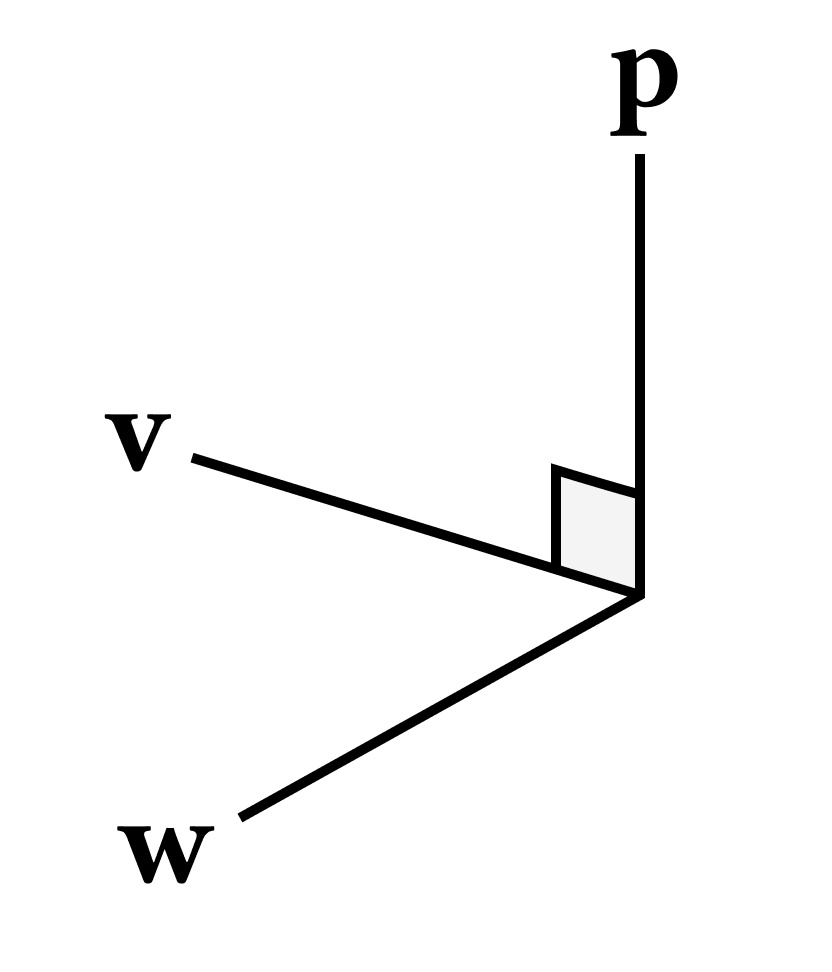
\includegraphics[width=0.2\textwidth]{resources/cross-product.png}
  \caption{Cross product of two vectors $v$ and $w$, resulting in a vector $p$ orthogonal to $v$ and $w$.}
  \label{fig:cross-product}
\end{figure}

\subsubsection{Matrices}

Matrices are used to represent transformations in computer graphics. A matrix can be defined using row-major order as:

\begin{equation}
  \label{eqn:matrix}
  M = \begin{bmatrix} M_{1,1} & M_{1,2} \\ M_{2,1} & M_{2,2} \end{bmatrix} = \begin{bmatrix} a & b \\ c & d \end{bmatrix}
\end{equation}

\subsubsection{Ray}

A ray can be defined as $r = (Q, d)$ where $Q$ is the origin vertex of the ray and $d$ is the direction vector.

\subsubsection{Triangle}

The triangle can be defined as $t = (Q, u, v)$ where $Q$ is the position of the triangle and $u$ and $v$ are vectors defining the triangle. See \autoref{fig:q-u-v-parameterization} for a visual representation.

\begin{figure}[H]
  \centering
  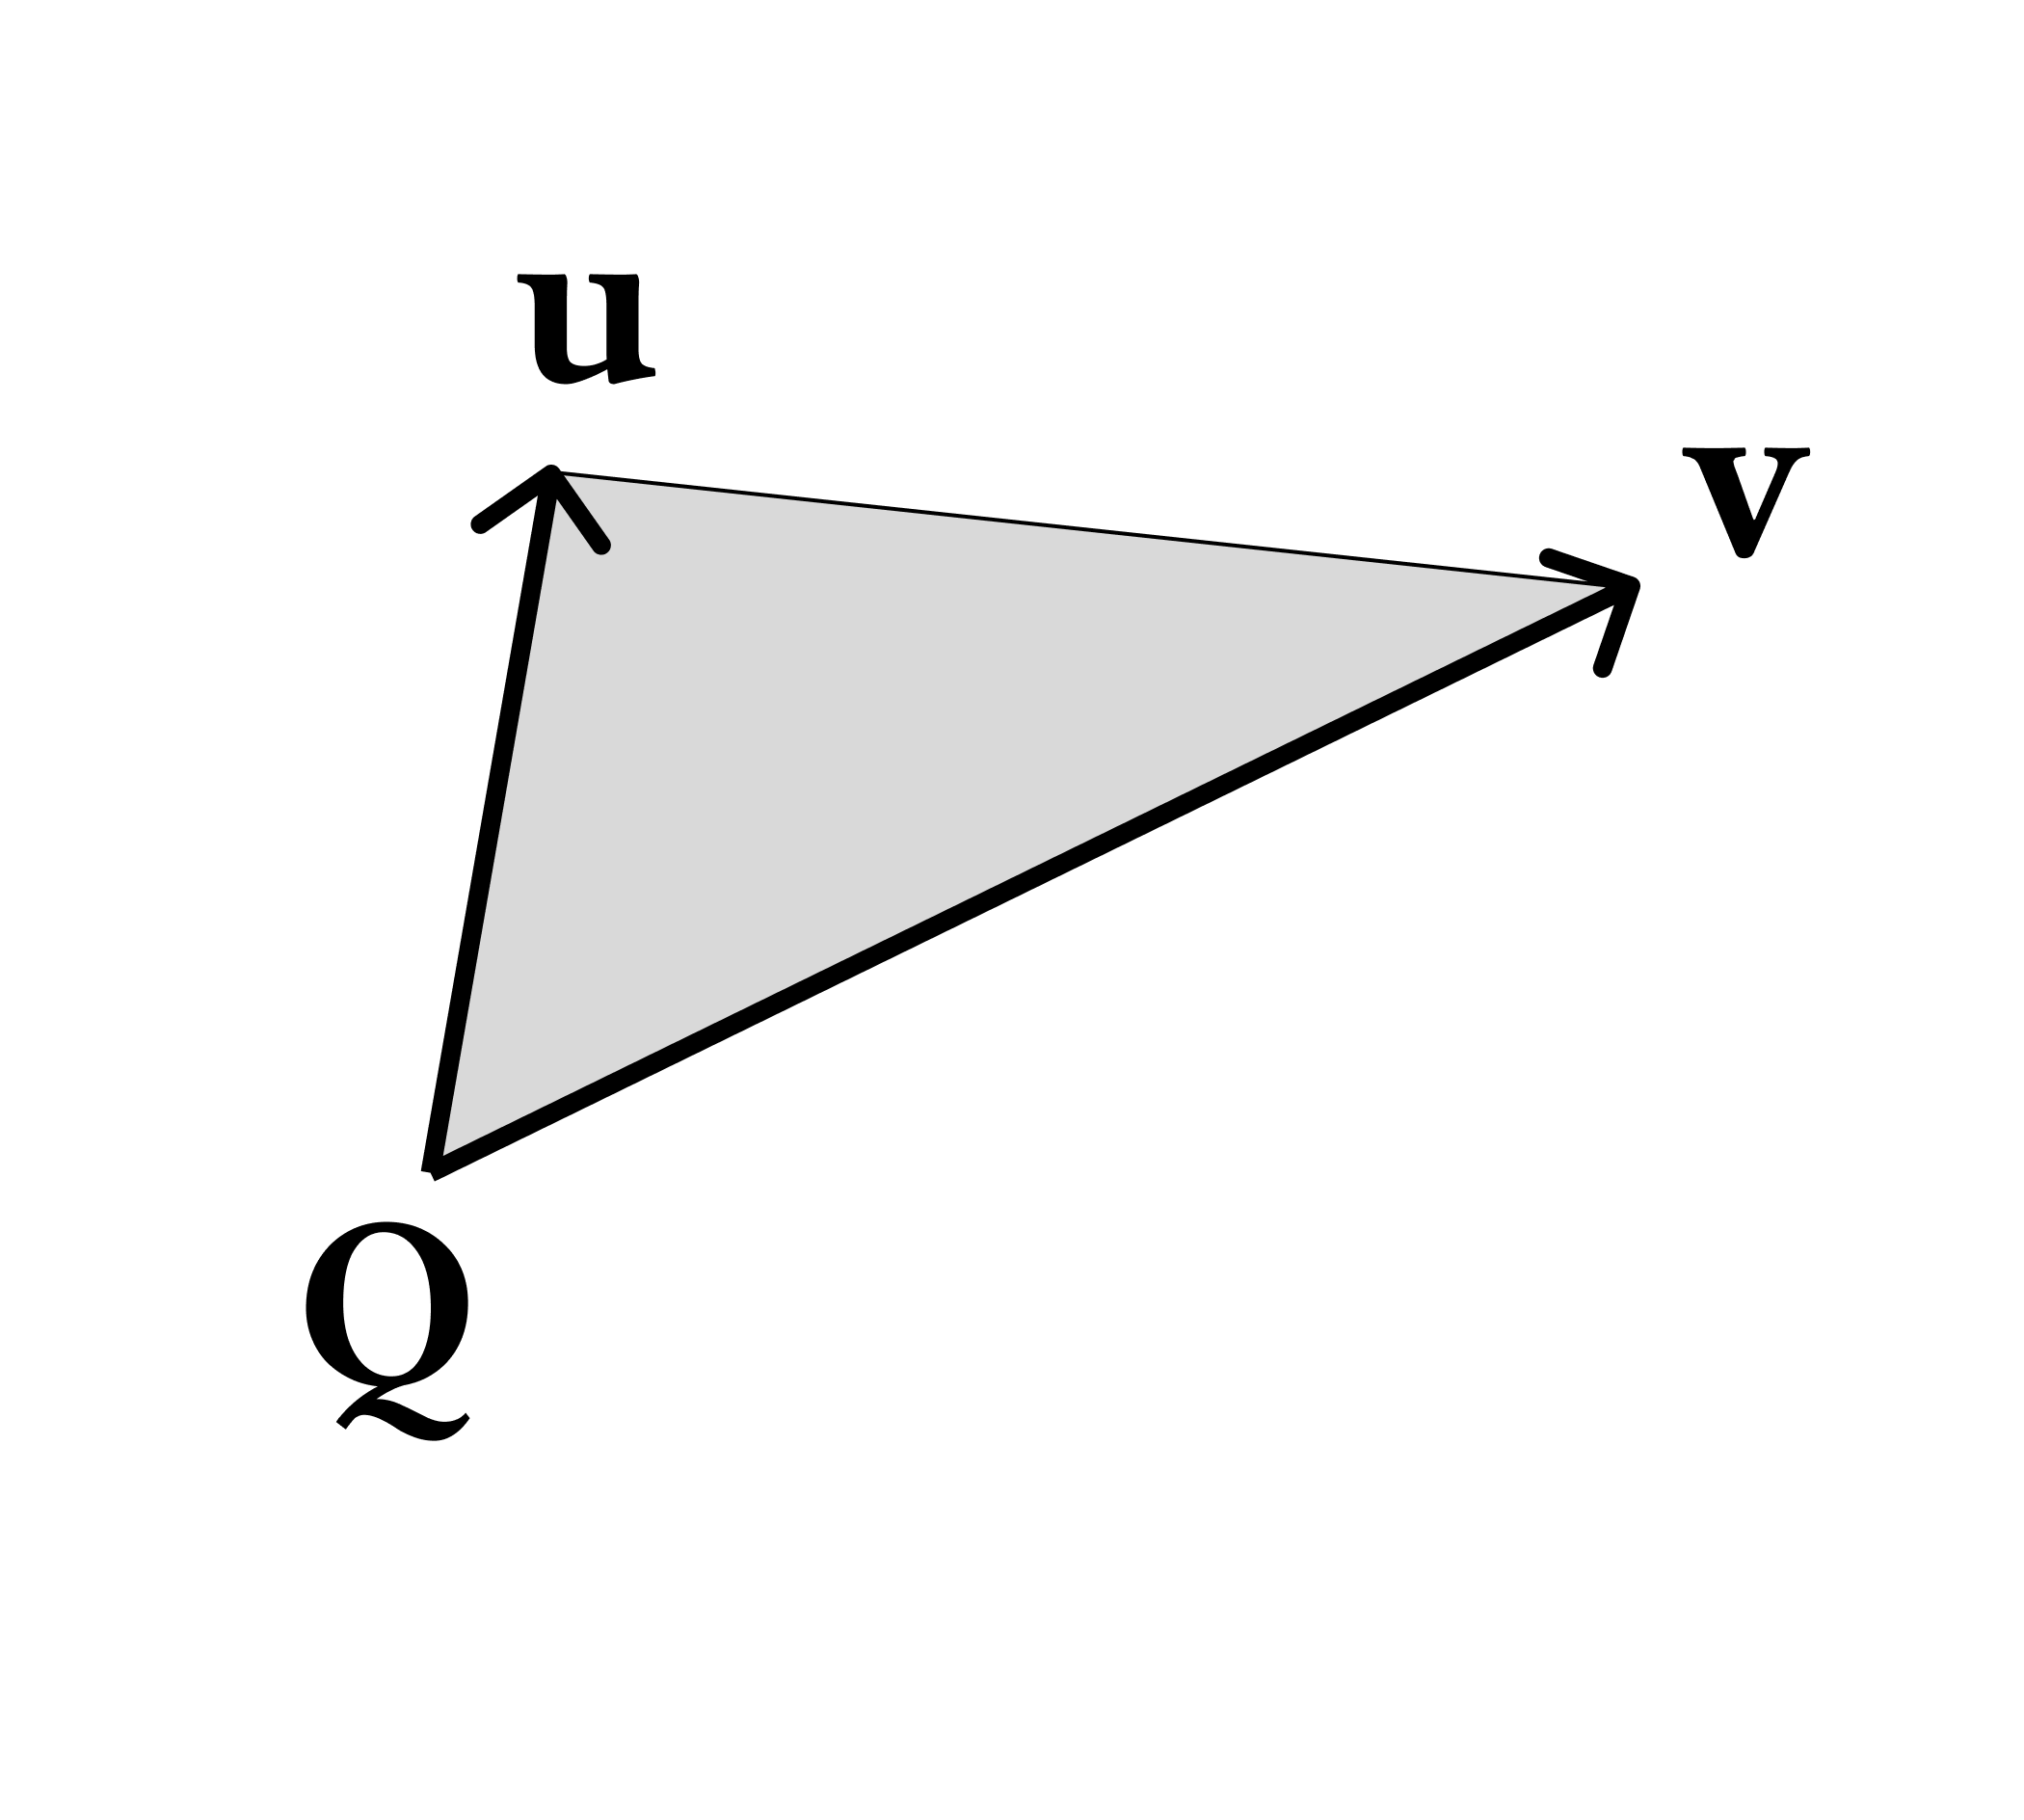
\includegraphics[width=0.25\textwidth]{resources/q-u-v-parameterization.png}
  \caption{Triangle defined using three vertices, $Q$ as the position and $u$,$v$ as direction vectors starting at $Q$.}
  \label{fig:q-u-v-parameterization}
\end{figure}

An alternative way to define a triangle is using three vertices, each in world space. The vertices can be defined as $v_1 = (x_1, y_1, z_1)$, $v_2 = (x_2, y_2, z_2)$ and $v_3 = (x_3, y_3, z_3)$. Converting between the two systems can be done using the following formulas:

\begin{equation}
  \label{eqn:triangle-vertices-to-q-u-v}
  Q = v_1
\end{equation}

\begin{equation}
  \label{eqn:triangle-vertices-to-q-u-v1}
  u = v_2 - v_1
\end{equation}

\begin{equation}
  \label{eqn:triangle-vertices-to-q-u-v2}
  v = v_3 - v_1
\end{equation}

A triangle has three normals, one for each vertex. The normal of a triangle can be calculated using the cross product of two edges of the triangle.

\subsubsection{Frustum}

The frustum is a geometric shape which is used to define the camera's view. See \autoref{fig:camera-frustum} for a visual representation.

\begin{figure}[H]
  \centering
  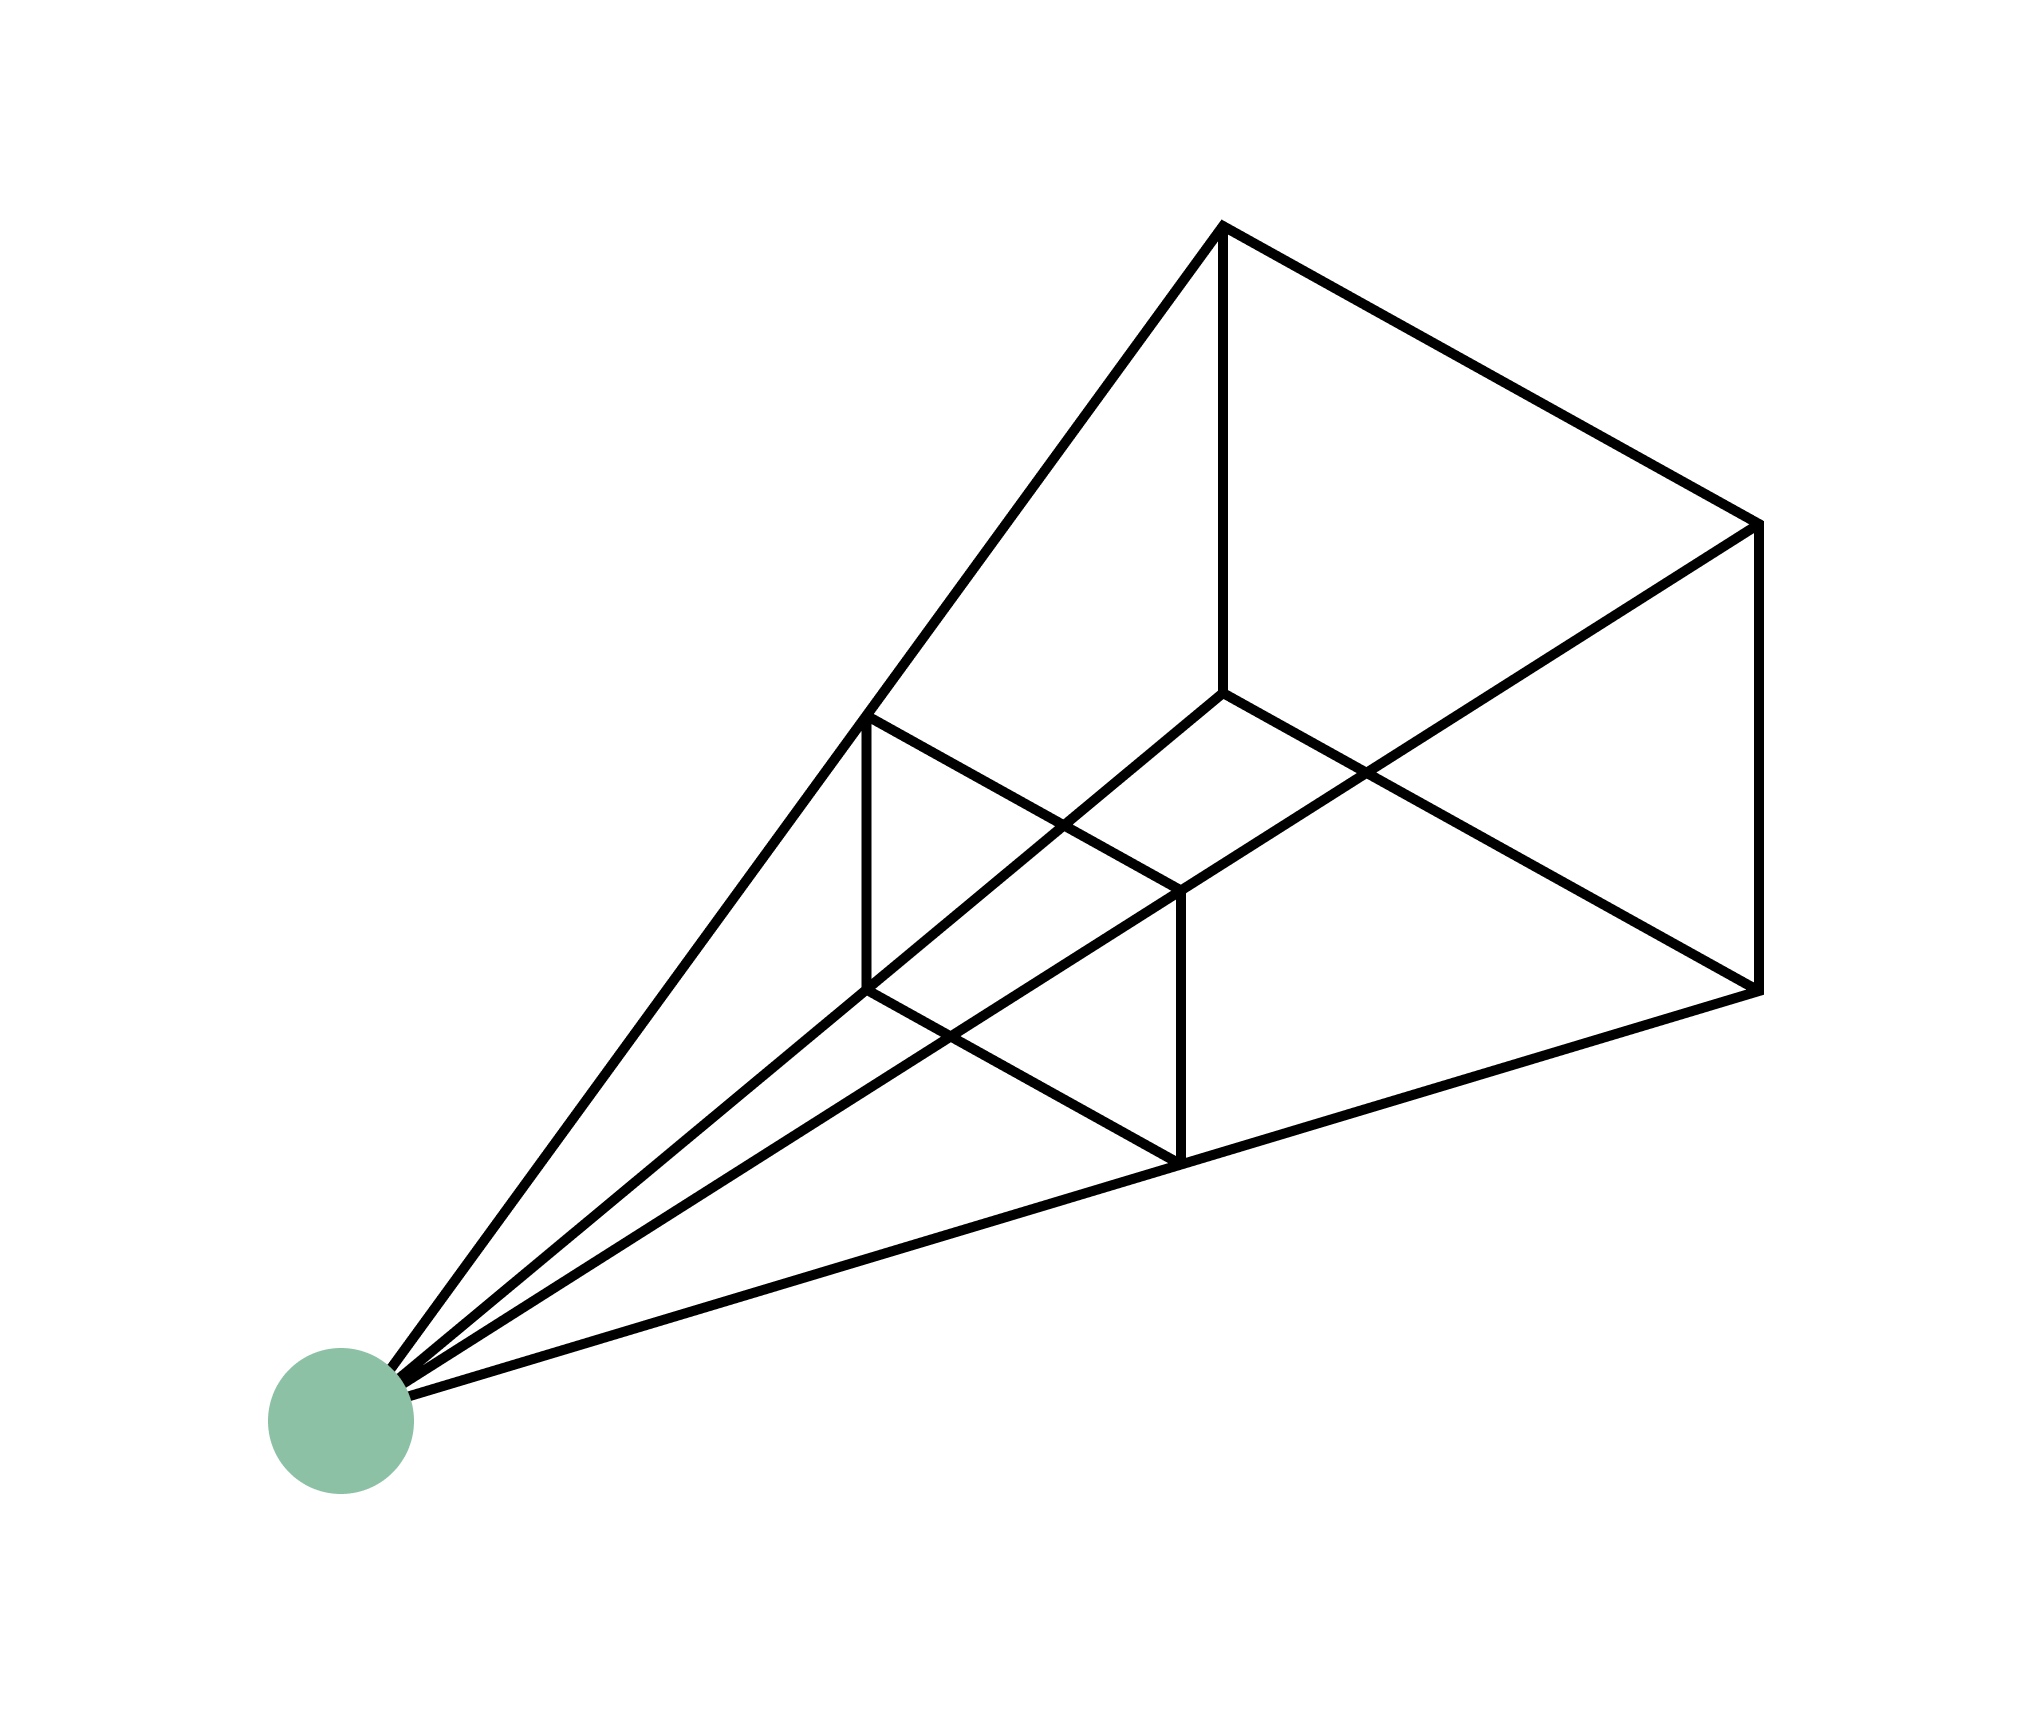
\includegraphics[width=0.25\textwidth]{resources/camera-frustum.png}
  \caption{Frustum shape, the green dot indicates the position of a camera in perspective projection.}
  \label{fig:camera-frustum}
\end{figure}

\section{Physics}

In order to generate images using computer graphics, understanding the physics is crucial. More specifically, the study of light and its perception is important. In physics, optics is the study of light. The field encompasses topics such as light propagation and optical properties of matter. Maxwell's equations are a set of equations in electromagnetism that describe the behavior of electromagnetic fields. Formulated by James Clerk Maxwell in the 19th century, they provide a mathematical framework for understanding the propagation of electromagnetic waves, including, but not limited to, visible light. Light can be described as a wave or as a particle, this is generally known as the wave-particle duality. \cite{fowles1989introduction}

\subsubsection{Reflection}

Reflection is the process of light bouncing off a surface. The angle of incidence equals the angle of reflection as visualized in \autoref{fig:reflection}. An example of such an effect can be seen when looking at a mirror.

\begin{figure}[H]
  \centering
  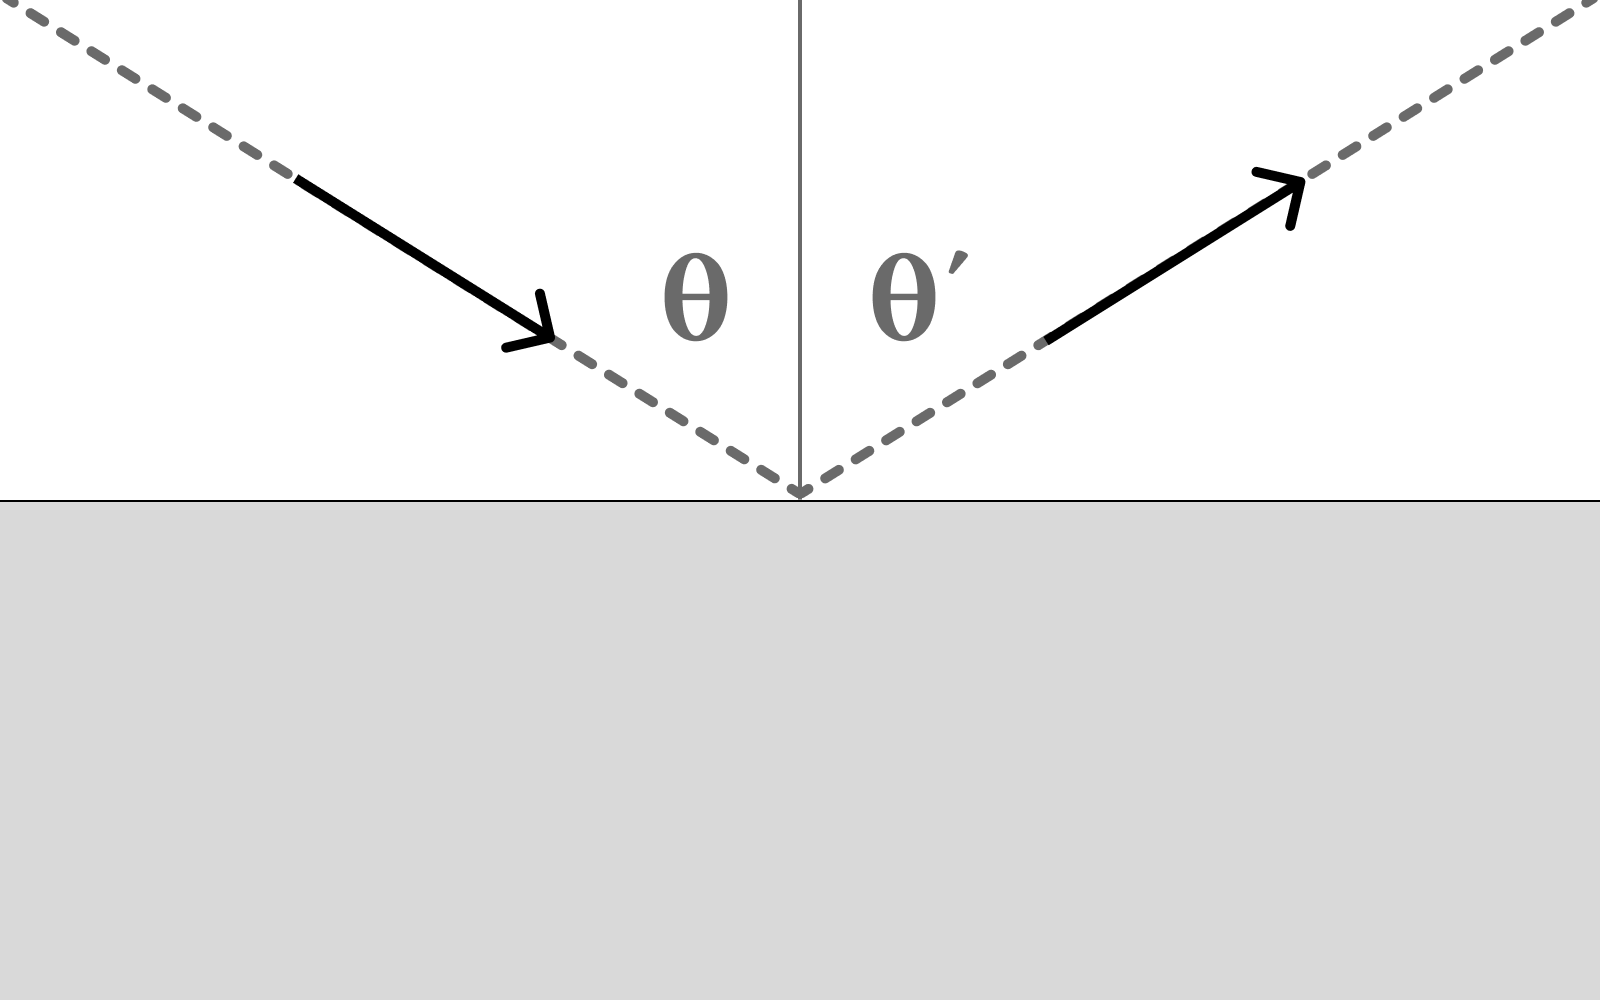
\includegraphics[width=0.4\textwidth]{resources/reflection.png}
  \caption{Reflection of light when hitting a surface.}
  \label{fig:reflection}
\end{figure}

This can be described using the law of reflection:

\begin{equation}
  \label{eqn:law-of-reflection}
  \theta = \theta'
\end{equation}

Where $\theta$ is the angle of incidence and $\theta'$ is the angle of reflection.

\subsubsection{Refraction}

Refraction is the bending of light when passing through a medium as visualized in \autoref{fig:refraction}. An example of such an effect is the distortion of underwater objects.

\begin{figure}[H]
  \centering
  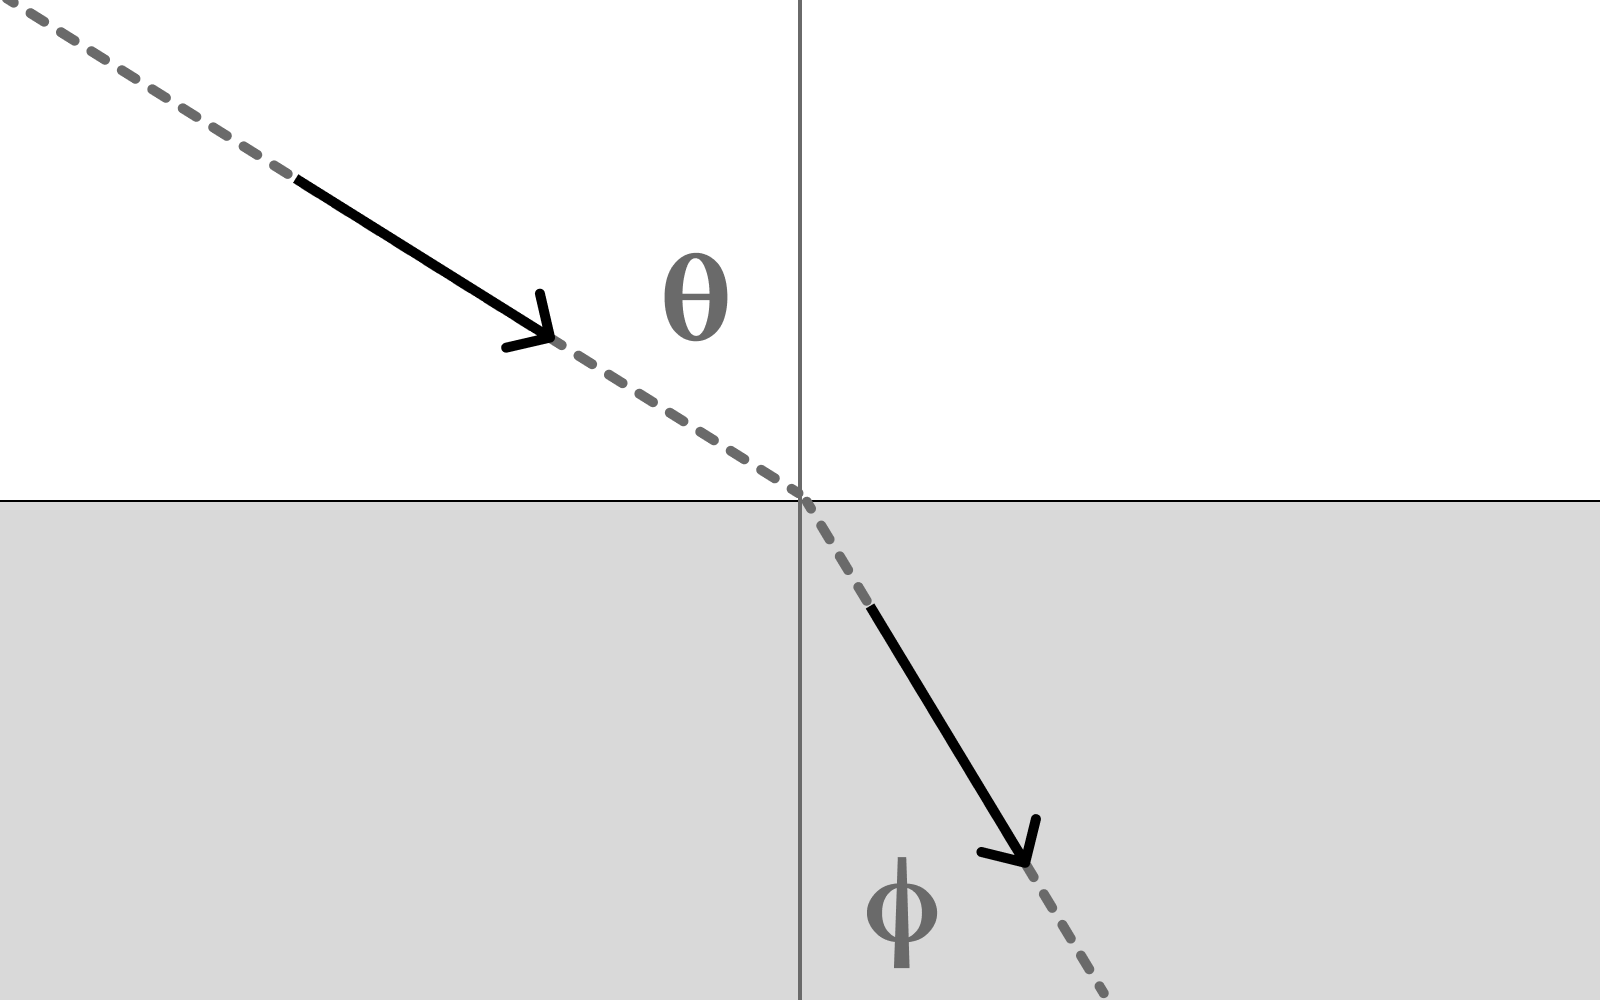
\includegraphics[width=0.4\textwidth]{resources/refraction.png}
  \caption{Refraction of light when passing through a medium.}
  \label{fig:refraction}
\end{figure}

It can roughly be defined by using Snell's law:

\begin{equation}
  \label{eqn:snells-law}
  \frac{\sin \theta}{\sin \phi} = n
\end{equation}

or in a more general form:

\begin{equation}
  \label{eqn:snells-law-general}
  n_1 \sin \theta = n_2 \sin \phi
\end{equation}

where $n_1$ and $n_2$ are the refractive indices of the two media and $\theta$ and $\phi$ are the angles of incidence and refraction respectively.

Leveraging Snell's law, fresnel equations can be derived which describe not only the refraction but also the reflection of light when passing through a medium.

\subsubsection{Isotropy}

Isotropy is a property of materials which have the same properties in all directions. An example of such a material is glass or water. Anisotropy on the other hand is a property of materials which have different properties in different directions. An example of such a material is wood or brushed metal. 

\section{Computer Graphics}
\label{ch:computerGraphics}

This section provides an overview of computer graphics, including its history, key concepts and applications.

Since the early days of computing, researchers have explored ways to process visual information using computers. While the field also encompasses aspects such as image processing or two-dimensional graphics, the main focus of this thesis is on three-dimensional computer graphics. While this includes topics such as animation, geometry processing, the main topics covered are geometry representation, rendering and shading.

\subsection{Global Illumination}

Research to render advanced lighting effects using computer graphics was conducated as early as the 1960s. One of the earliest papers describing approaches to render shadow casting was written as early 1968 by Appel \cite{appel1968shading}. In order to describe the phenomena, encountered in real 

The term global illumination was coined by Whitted in 1979 \cite{whittedGlobalIllumination}. It describes a complete shading model that simulates real lighting and reflection as accurately as possible \cite{whitted2020OriginsOfGlobalIllumination}.

Simulating real lighting includes effects such as:

\begin{itemize}
  \item{Shadow Casting} — The absence of light as obstructed by other objects.
  \item{Reflection} — As in the case of mirror-like objects, but also for specular and metallic reflection.
  \item{Refraction} — As encountered when light passes through water.
  \item{Color Bleeding} — Special type of reflection, where a surface is colored by reflection of colored light.
  \item{Ambient Occlusion} — Special type of shadow casting, where light transport as impacted by nearby objects is considered.
\end{itemize}

\todo{Add illustrations for effects}

\subsection{Rasterization}
\label{ch:rasterizationTheory}

In order to visualize 3D scenes using a computer, different rendering approaches have been developed. Two of the most common approaches are rasterization and ray tracing and will be described in more detail in the following sections.

Rasterization is a rendering technique which maps the geometry of a 3D scene onto a 2D plane. Historically, the technique has been widely adopted in real-time rendering due to its efficiency. However, there are inherent limitations in terms of realism.

One of the main limitations is the lack of support for global illumination.

\subsubsection{Limitations}

\subsubsection{Advanced Techniques}

Various methods have been developed to address these limitations, including pre-baked shadow, environment \cite{greene1986environment} and light maps; screen space reflections (SSR) \cite{screenSpaceReflectionsStackowiak}; screen space ambient occlusion (SSAO) \cite{bavoil2008ssao}; and screen space directional occlusion (SSDO) \cite{ritschel2009ssdo}.

To obtain reflections, one frequently used technique is multi-pass rendering. The idea is to first render the scene from the perspective of the reflective object and then render a second pass from the camera while leveraging the first pass as a texture.

These approaches induce complexity and can be computationally expensive. An alternative technique which resembles reality more closely could alleviate these issues: Ray Tracing.

\subsection{Ray Tracing}
\label{ch:rayTracingTheory}

Ray Tracing is a rendering technique which simulates light transport in a scene. The main idea is to cast rays from the camera into the scene and compute the color of the object the ray intersects with. By adding additional bounces of the light ray, the technique can simulate global illumination.

Early algorithms were based on recursive ray tracing \cite{whittedGlobalIllumination}. These algorithms determine intersection with geometry and iteratively generate branches as shown in \autoref{fig:recursiveRayTracing}.

\begin{figure}[H]
  \centering
  \begin{subfigure}[b]{0.45\textwidth}
      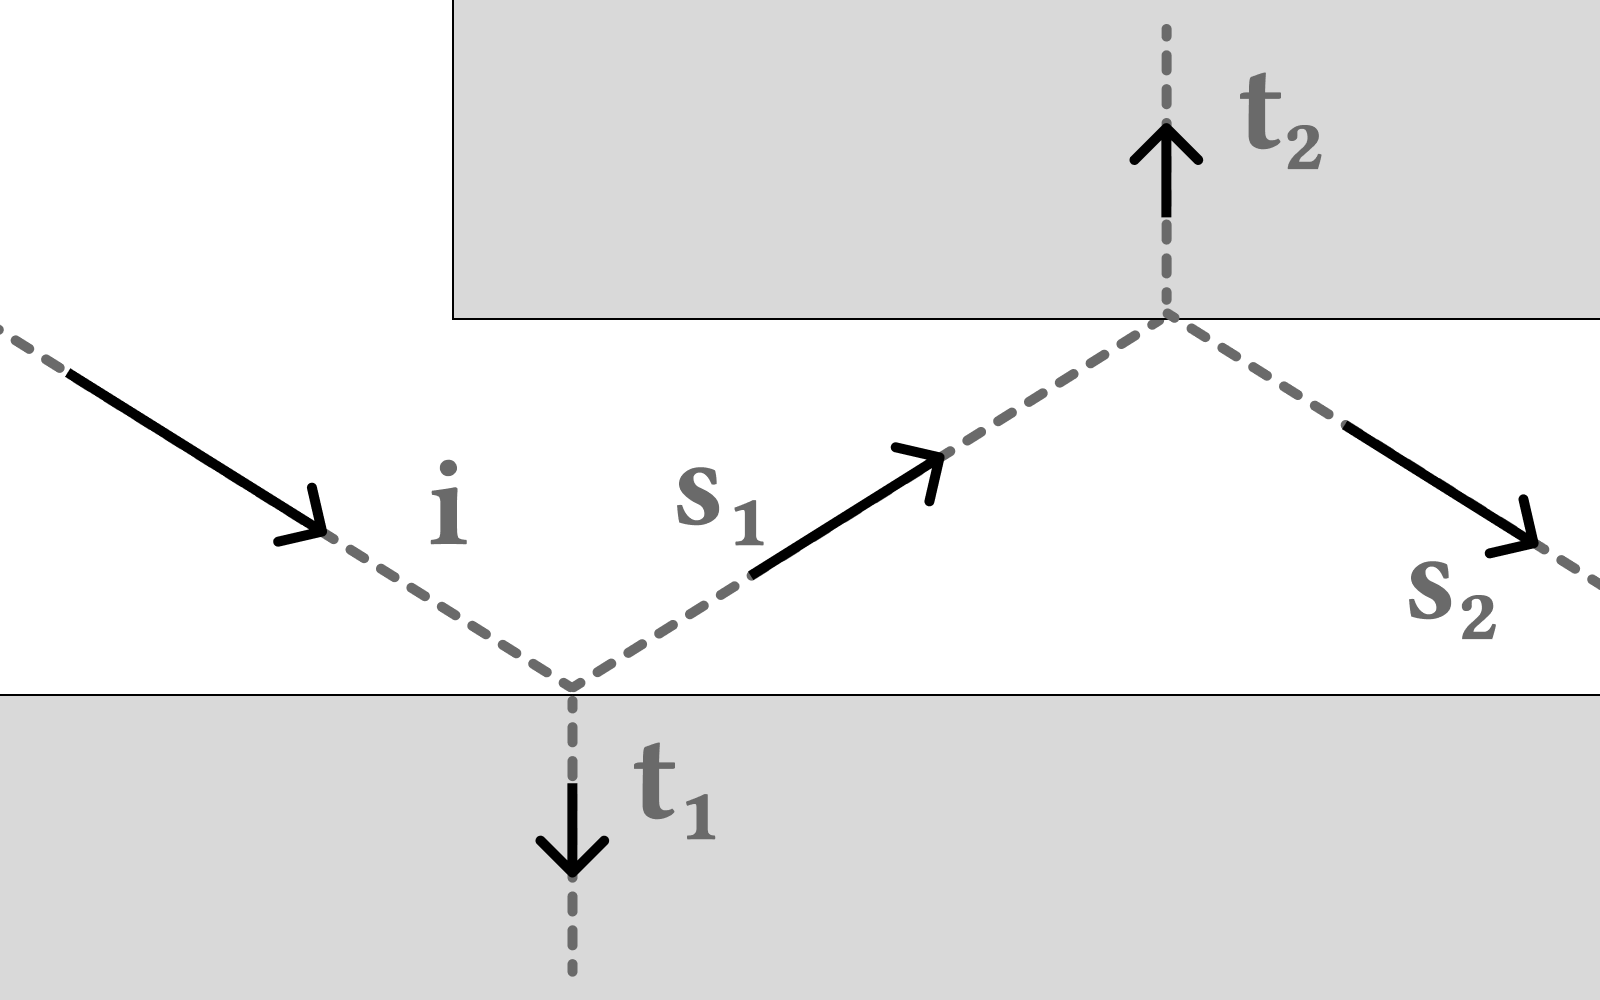
\includegraphics[width=\textwidth]{resources/recursive-ray-tracing-visualized.png}
      \caption{Incident ray hitting a surface generating two branches, $s_1$ and $t_1$.}
      \label{fig:recursiveVisualized}
  \end{subfigure}
  \hfill
  \begin{subfigure}[b]{0.3\textwidth}
    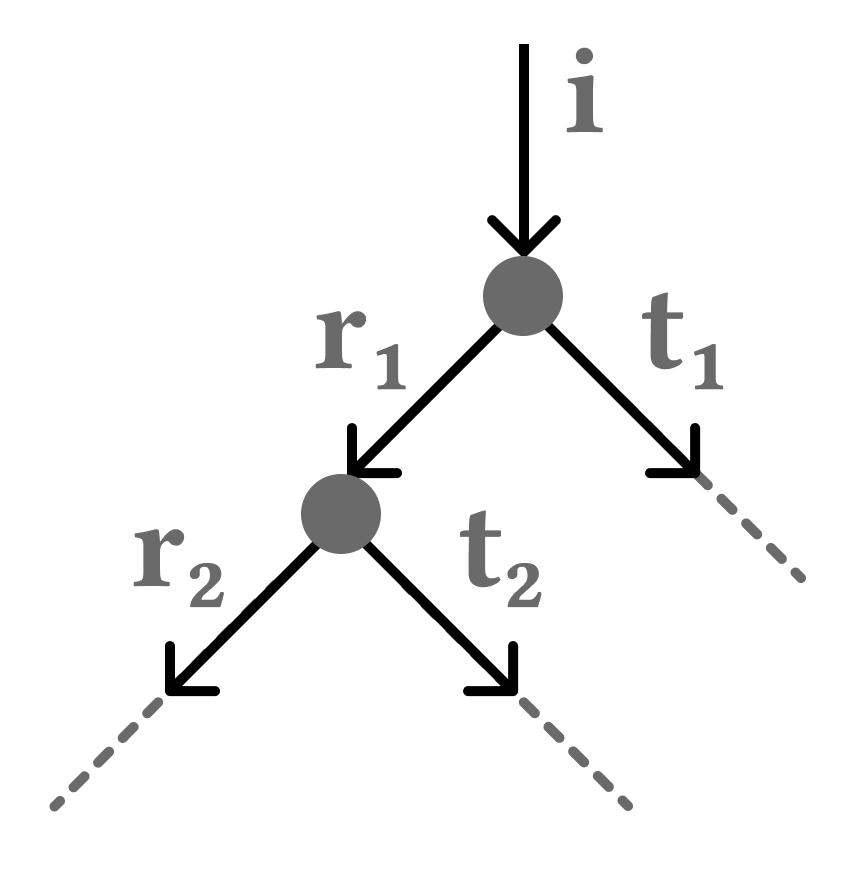
\includegraphics[width=\textwidth]{resources/recursive-ray-tracing-tree.png}
    \caption{Recursive ray tracing visualized as tree structure}
    \label{fig:recursiveTree}
  \end{subfigure}
  \caption{Recursive ray tracing as described by Whitted \cite{whittedGlobalIllumination}.}
  \label{fig:recursiveRayTracing}
\end{figure}

Due to the computational complexity of these early algorithms, ray tracing was not widely adopted until the 1980s.

During these years, one of the main concepts was the introduction of the rendering equation by Kajiya in 1986 in a paper which also coined the term path tracing. Generally, path tracing can be seen as a Monte Carlo integration of the rendering equation which is defined as:

\begin{equation}
  \label{eqn:rendering-equation}
  I(x, x') = g(x, x') [\epsilon(x, x') + \int_{S} p(x, x', x'')I(x', x'')dx'']
\end{equation}

where $I(x, x')$ is the radiance from point $x$ to point $x'$. $x$ for example being the camera position and $x'$ the intersected object. $g(x, x')$ is a geometry term determining how much light is transmitted. This depends on the distance and possibly occlusions such as transparent surfaces. $\epsilon(x, x')$ is the emitted radiance, generally used for light sources. The integral term is taken over $S$ = $\cup S_i$ which is the union of all surfaces. $p(x, x', x'')$ is the bidirectional reflection function, which describes how light from all possible directions $x''$ is reflected at the surface. \cite{kajiya1986rendering}

Some of the first widely used ray tracing software was POV-Ray, which was released in 1991 \cite{POV_Ray_Documentation}. Blue Moon Rendering Tools (\gls{BMRT}) \cite{bmrt}, a \fGls{RenderMan}{A rendering software for photorealistic 3D rendering developed by Pixar} compliant renderer, was released in the mid 90s and was one of the first ray tracing renderers to be used in the industry. In 2003 \gls{RenderMan} included ray tracing capabilities \cite{RenderMan_11_Release_Notes}.

Further research into light transport techniques such as bidirectional light transport or Metropolis Light Transport has been conducted in the 1990s \cite{veachMonteCarloLightTransport}.

\subsubsection{Monte Carlo Ray Tracing}
\subsubsection{Intersection Testing}

When casting a ray into the scene, the first step in a ray tracer is to determine where the ray intersects with the geometry of the scene.

A brute force approach could be to determine the intersection distance for each object to the ray and picking the one with the lowest distance. Given the fact, that common objects consist of thousands of triangles ($n$) and ray tracing many rays, this approach is not efficient as it would worst case require $O(n)$ intersection tests for each ray.

In order to accelerate the intersection testing, various approaches have been developed.

The bounding volume hierarchy (\gls{BVH}) is an acceleration structure which is leveraged to speed up the ray intersection tests. This method is widely used in ray tracing and has been studied for a long time \cite{rubinWhittedBvh}. The core idea is to group adjacent objects in a bounding volume and structure the hierarchy in a way that all child elements of a node are contained in the bounding volume of the parent node. This allows for early rejection of branches which are not intersected by the ray. By employing a \gls{BVH}, the number of intersection tests ($n$) can be reduced from $O(n)$ to $O(log(n))$.

A bounding box ($b$) can be defined as $b = (min, max)$ where $min$ and $max$ are the minimum and maximum vertices of the bounding box. The boxes are then grouped into a hierarchy where the maximum and minimum vertices of the children define the bounding box of the parent. This is visualized in \autoref{fig:bvhVisualized}. Good performance of the \gls{BVH} depends on the quality of the hierarchy. A badly constructed \gls{BVH} can lead to a higher number of intersection tests as visualized in \autoref{fig:bvhBad} because intersections need to be tested against all elements: three bounding boxes and four triangles. For a well-constructed \gls{BVH}, the algorithm can reduce the number of intersection tests as visualized in \autoref{fig:bvhGood} by doing the minimum amount of intersection tests: $b_1$, which intersects, $b_2$ which can be discarded after checking and then $b_3$ necessitates further intersection tests for the two contained triangles. For such a small number of triangles, the overhead of the \gls{BVH} exceeds the benefits, but for larger scenes, the performance gain is significant as the amount of tests can be halved for well-balanced trees.

\begin{figure}[H]
  \centering
  \begin{subfigure}[b]{0.45\textwidth}
      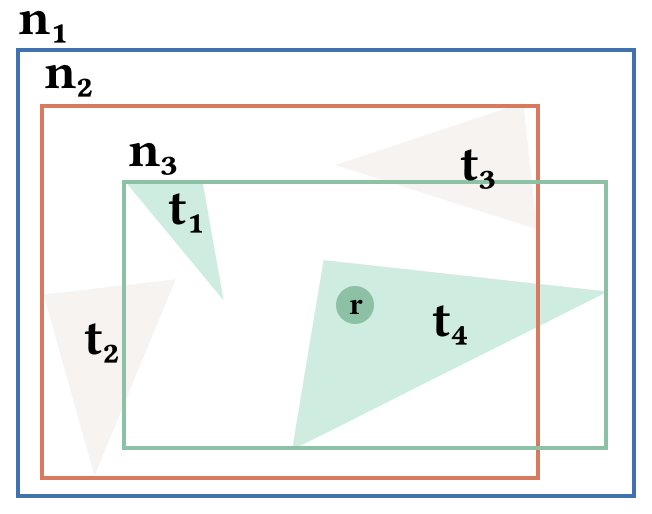
\includegraphics[width=\textwidth]{resources/bvh-bad-visualized.png}
      \caption{Badly-constructed \gls{BVH} which requires seven intersection tests for $r$, essentially testing against all objects.}
      \label{fig:bvhBad}
  \end{subfigure}
  \hfill
  \begin{subfigure}[b]{0.45\textwidth}
    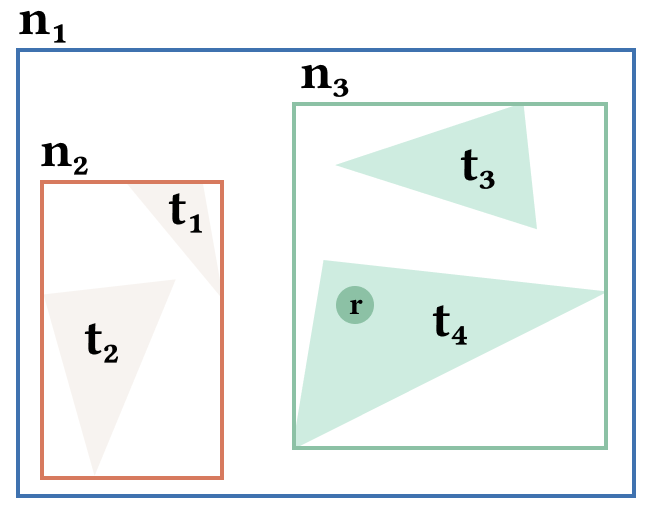
\includegraphics[width=\textwidth]{resources/bvh-good-visualized.png}
    \caption{Well-constructed \gls{BVH} which reduces the required intersection tests for $r$ to four.}
    \label{fig:bvhGood}
  \end{subfigure}
  \caption{Sample 2D \gls{BVH} visualization which contains four triangles ($t_1$ to $t_4$) and their corresponding bounding boxes $b_1$ as parent and $b_2$ as well as $b_3$ as the children. $b_1$ is visualized bigger than need be to improve readability. The color of the triangles indicates to which bounding box they belong. $r$ indicates the ray to be tested for intersection.}
  \label{fig:bvhVisualized}
\end{figure}

\subsubsection{Importance Sampling}

\subsubsection{Hybrid Approaches}

Ray Tracing and Rasterization are not mutually exclusive. Hybrid approaches have been developed which leverage a multi-paradigm approach. One such example is PICA PICA, a real-time ray tracing experiment developed by Nvidia \cite{hybridRenderingBarreBrisebois2019}. The rendering pipeline is split into multiple stages, consisting of global illumination, shadow, reflection, direct lighting. Each stage could be implemented using different techniques where the strategy could be chosen based on the requirements of the scene as well as the available computational resources.

\subsection{Common Techniques}

While rasterization and ray tracing are inherently different techniques, they face similar challenges. Notable frequently encountered challenges and their differences in rasterization and ray tracing are discussed in the following sections.

\subsubsection{View Projection}

In order to render an image, a virtual camera needs to be defined. Given a vertex as $p = (x, y, z)$, the view projection is responsible for transforming the vertex into normalized device coordinates. The view projection matrix is a 4x4 matrix which depends on the projection type.

Depending on the use case, different types of camera projection can be used. The most common types are perspective and orthographic projection. Perspective projection simulates the way the human eye perceives the world, objects which are further away appear smaller. Whereas orthographic projection does not take the distance into account and objects appear the same size regardless of their distance. Orthographic projection is frequently used in domains such as architecture.

These two projection types differ in the view projection matrix. For perspective projection, the following parameters need to be defined:

\begin{description}
    \item[near ($n$)] The distance from the camera to the near clipping plane.
    \item[far ($f$)] The distance from the camera to the far clipping plane.
    \item[fov ($\theta$)] The \textit{field of view} angle, measured in degrees.
    \item[aspect ratio ($r$)] The ratio of the viewport's width to its height.
\end{description}

The clipping plane parameters $n$ and $f$ are primarily used in rasterization to determine the camera frustum. Using equations \ref{eqn:perspectiveProjectionHeight} and \ref{eqn:perspectiveProjectionWidth}, the view projection matrix $P$ for perspective projection is defined in equation \ref{eqn:perspectiveProjectionMatrix}.

\begin{equation}
    \label{eqn:perspectiveProjectionHeight}
    h = 2n \cdot \tan(\frac{\theta}{2} \underbrace{\pi / 180}_{\text{deg to rad}})
\end{equation}

\begin{equation}
    \label{eqn:perspectiveProjectionWidth}
    w = rh
\end{equation}

\begin{equation}
    \label{eqn:perspectiveProjectionMatrix}
    P = 
    \begin{bmatrix}
        \frac{2n}{w} & 0 & 0 & 0 \\
        0 & \frac{2n}{h} & 0 & 0 \\
        0 & 0 & -\frac{f + n}{f - n} & -\frac{2fn}{f - n} \\
        0 & 0 & -1 & 0
    \end{bmatrix}
\end{equation}

The elements $P_{1,1}$ and $P_{2,2}$ adjust the field of view and therefore the perspective effect. The elements $P_{3,3}$, $P_{3,4}$ and $P_{4,3}$ adjust the near and far clipping planes. In comparison to rasterization, the view projection matrix is used differently in ray tracing. In rasterization, every vertex is transformed by the view projection matrix. In ray tracing, the view projection matrix is only applied to the camera rays.

For ortographic projection, no such projection matrix is required in ray tracing. Instead, parallel rays are cast from the camera grid.

\subsubsection{Random Number Generator}

  
To simulate light transport, the path tracer needs to pick random directions. Generating a random direction vector, defined as $v = (x, y, z)$, can be achieved by picking three random numbers independent of one another. This pivotal part of path tracing is done using a random number generator (\gls{RNG}). In rasterization, the necessity for \gls{RNG} is less common, but may still be required for certain effects. Unlike other programming languages, \gls{WGSL} does not have a built-in \gls{RNG}. Therefore, a custom \gls{RNG} is required. There are a variety of \gls{RNG}s available which differ in important characteristics. Some of the characteristics to consider when choosing a suitable \gls{RNG} are:

\begin{itemize}
    \item{Statistical Quality} – The \gls{RNG} should generate numbers that are statistically random. This means that the numbers should be uniformly distributed and have a low correlation between them.
    \item{Period} – The length of the cycle before the sequence of generated numbers starts to repeat itself.
    \item{Time Performance} – The time it takes to generate a random number. This is influenced by the algorithm as well as the hardware which may support dedicated instructions.
    \item{Space Usage} – The amount of memory required to store state.
\end{itemize}

Based on the use case, other factors such as prediction difficulty or others such as highlighted by O’Neill \cite{o2014pcg} may be important. Cryptography for example requires randomness of the \gls{RNG} to prevent an adversary from predicting secret keys. Options to generate the randomness require additional signals \cite{randomnessCryptography} or may require special hardware such as LavaRand \cite{cloudflareLavaRand}. Many generators are pseudorandom generators. These generators are deterministic and require a seed to start the sequence. For crypographically secure generators, the seed must be random.
However, for a path tracer, there is no need for cryptographic security. Instead, it is more important to have high performance and having a long period to avoid repetition. Therefore, a pseudorandom number generator with non-cryptographically secure seed is used.

One option for such a pseudorandom generator is using Xorshifts such as described by Marsaglia \cite{marsaglia2003xorshift}. The algorithm can be defined as shown in Figure \ref{code:xorShift}. $x$ is the state of the \gls{RNG} and $a$, $b$ and $c$ are constants which are chosen to achieve good statistical properties. Frequent choices for these constants are $a = 13$, $b = 17$ and $c = 5$.

\begin{figure}[H]
\begin{lstlisting}[style=wgsl]
x ^= x << a;
x ^= x >> b;
x ^= x << c;
\end{lstlisting}
\caption{Xorshift \gls{RNG} implementation in \gls{WGSL}.}
\label{code:xorShift}
\end{figure}

Alternatives to Xorshift are available, such as the Mersenne Twister \cite{rngMersenneTwister}. The Mersenne Twister is a pseudorandom number generator which has a long period and good statistical properties. However, it is slower than Xorshifts \cite{o2014pcg}. More recently, \fGls{PCG}{Permuted Congruential Generator, a family of random number generators} has been proposed as an alternative to these options. \gls{PCG} is a family of fast generators.

\subsubsection{Anti-aliasing}
\label{sec:anti-aliasing}

Aliasing is a common issue in computer graphics. It occurs when the resolution of the screen is not sufficient to represent the scene accurately. One such example is jagged edges on diagonal lines. Anti-aliasing techniques can be employed to reduce the effect. The negative effect of aliasing is demonstrated in \autoref{fig:aliasingA}.

\begin{figure}[H]
    \centering
    \begin{subfigure}[b]{0.45\textwidth}
        
\includegraphics[width=\textwidth]{resources/aliasing.png}
        \caption{Rendering showing aliasing.}
        \label{fig:aliasingA}
    \end{subfigure}
    \hfill
    \begin{subfigure}[b]{0.45\textwidth}
        
\includegraphics[width=\textwidth]{resources/anti-aliasing.png}
        \caption{Rendering with anti-aliasing applied.}
        \label{fig:aliasingB}
    \end{subfigure}
    \caption{The two images show the effect of aliasing and anti-aliasing.}
    \label{fig:aliasing}
\end{figure}

In ray tracing, aliasing can be alleviated by randomizing the direction of the rays for the different samples taken. The result of applying anti-aliasing can be seen in \autoref{fig:aliasingB}.

In rasterization, similar solution strategies can be employed. Supersampling is a common technique which renders the scene at a higher resolution and then downsamples the image by averaging the colors of the pixels. More elaborate techniques such as deep learning super sampling (DLSS) implemented by Nvidia \cite{nvidiaDlss} can be used to further improve the quality of the image in real-time rendering.

\section{Physically Based Rendering}

Defining the geometry is one part of the equation. Another major part is defining materials. Materials define how a surface interacts with light. The core idea of physically based rendering (\gls{PBR}) is to simulate the interaction of light using physical models. Instead of fine-tuning parameters for a specific look and feel and having to adjust based on desired lighting situations, \gls{PBR} aims to define a material which behaves consistently in different lighting situations.

Research into \gls{PBR} has been conducted for a similar amount of time as ray tracing. And just like ray tracing, the computational complexity of the algorithms has limited the adoption of \gls{PBR} in real-time rendering for a long time \todo{Quote some early adopters of 2000s?}. \gls{PBR} has generally coincided with the rise of ray tracing as it is a natural fit for the physics based rendering approach. However, \gls{PBR} and ray tracing are not mutually dependent as \gls{PBR} can be used in rasterization as well.

In contrast to how ray tracing is inherently addressing shortcomings of rasterization by leveraging an entirely different approach, \gls{PBR} is a more incremental improvement extending existing shading techniques with more sophisticated models.

In general, there is no \gls{PBR} standard. Instead, a variety of different models have been developed over time. In recent years however, a convergence towards a common set of principles has been observed. Nevertheless, certain aspects of \gls{PBR} are found in most models.

\subsection{BxDF}

The definition of the bidirectional distribution functions (BxDF) is a key concept in PBR. The $x$ stands for the different kinds of distributions to consider. In general, the functions describe how light is reflected or transmitted. The two functions are usually abbreviated as BRDF, the r standing for reflectance, and BTDF, the t standing for transmittance.

These functions define the distribution of light in different directions. Samples of different kinds of reflectance distributions can be seen in \autoref{fig:brdf}. Many objects exhibit a combination of different reflectance distributions.

\begin{figure}[H]
  \centering
  \begin{subfigure}[b]{0.45\textwidth}
      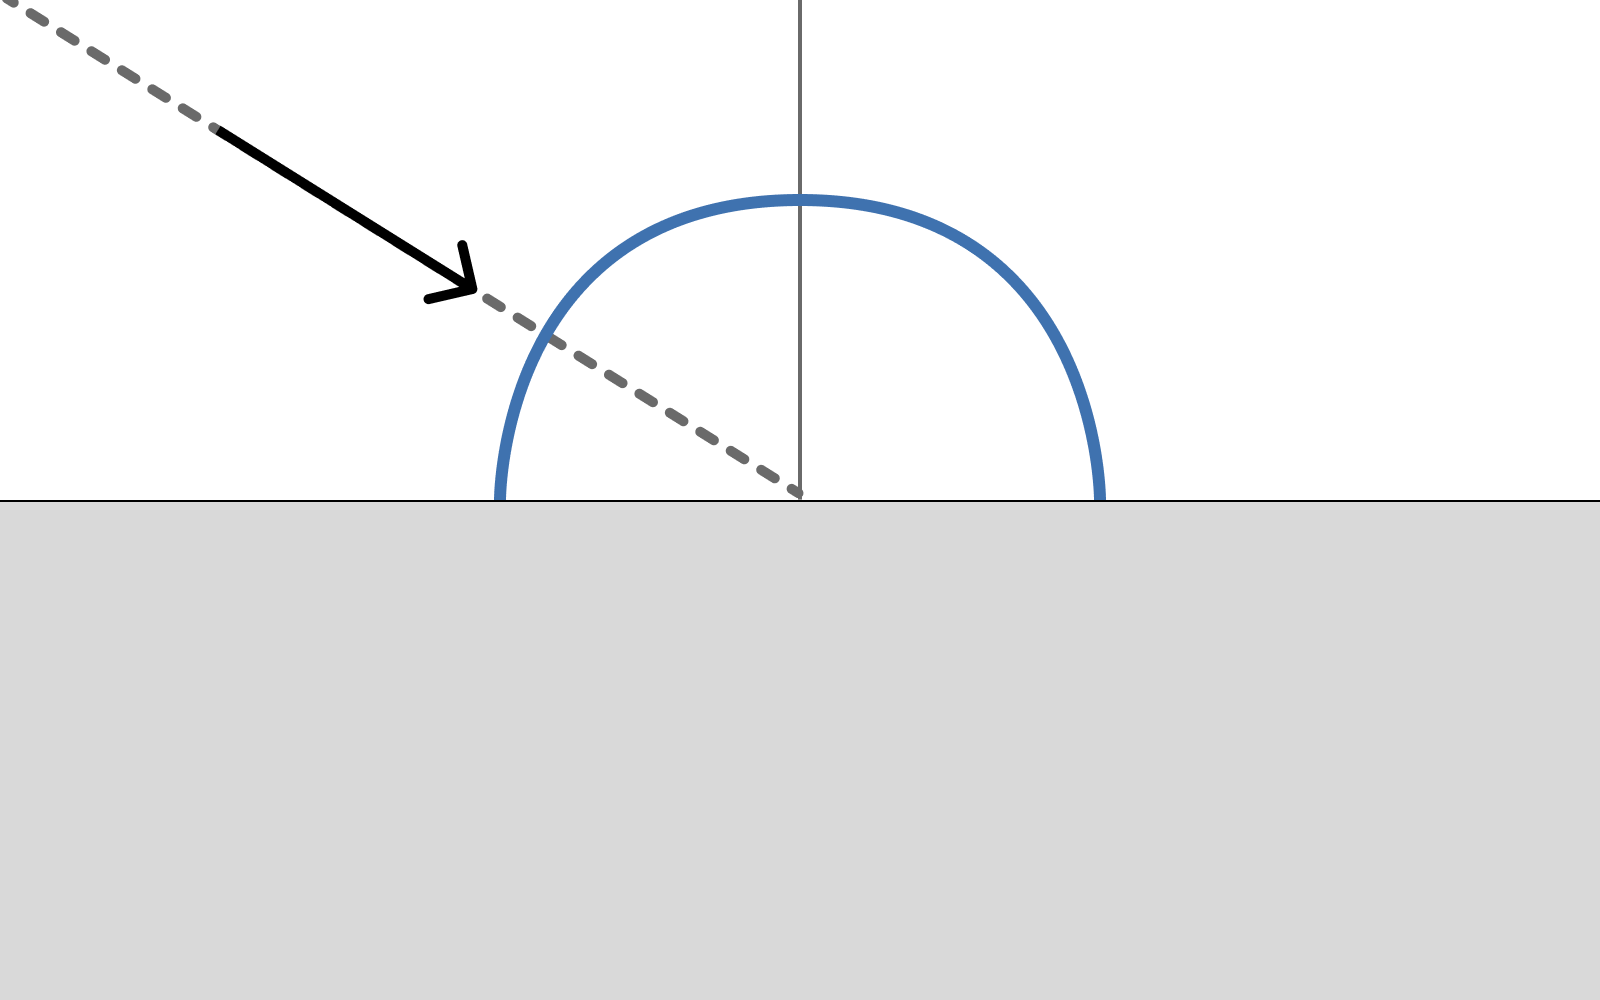
\includegraphics[width=\textwidth]{resources/reflection-diffuse.png}
      \caption{Diffuse reflection, as can be encountered in materials such as a paper.}
      \label{fig:reflectionDiffuse}
  \end{subfigure}
  \hfill
  \begin{subfigure}[b]{0.45\textwidth}
      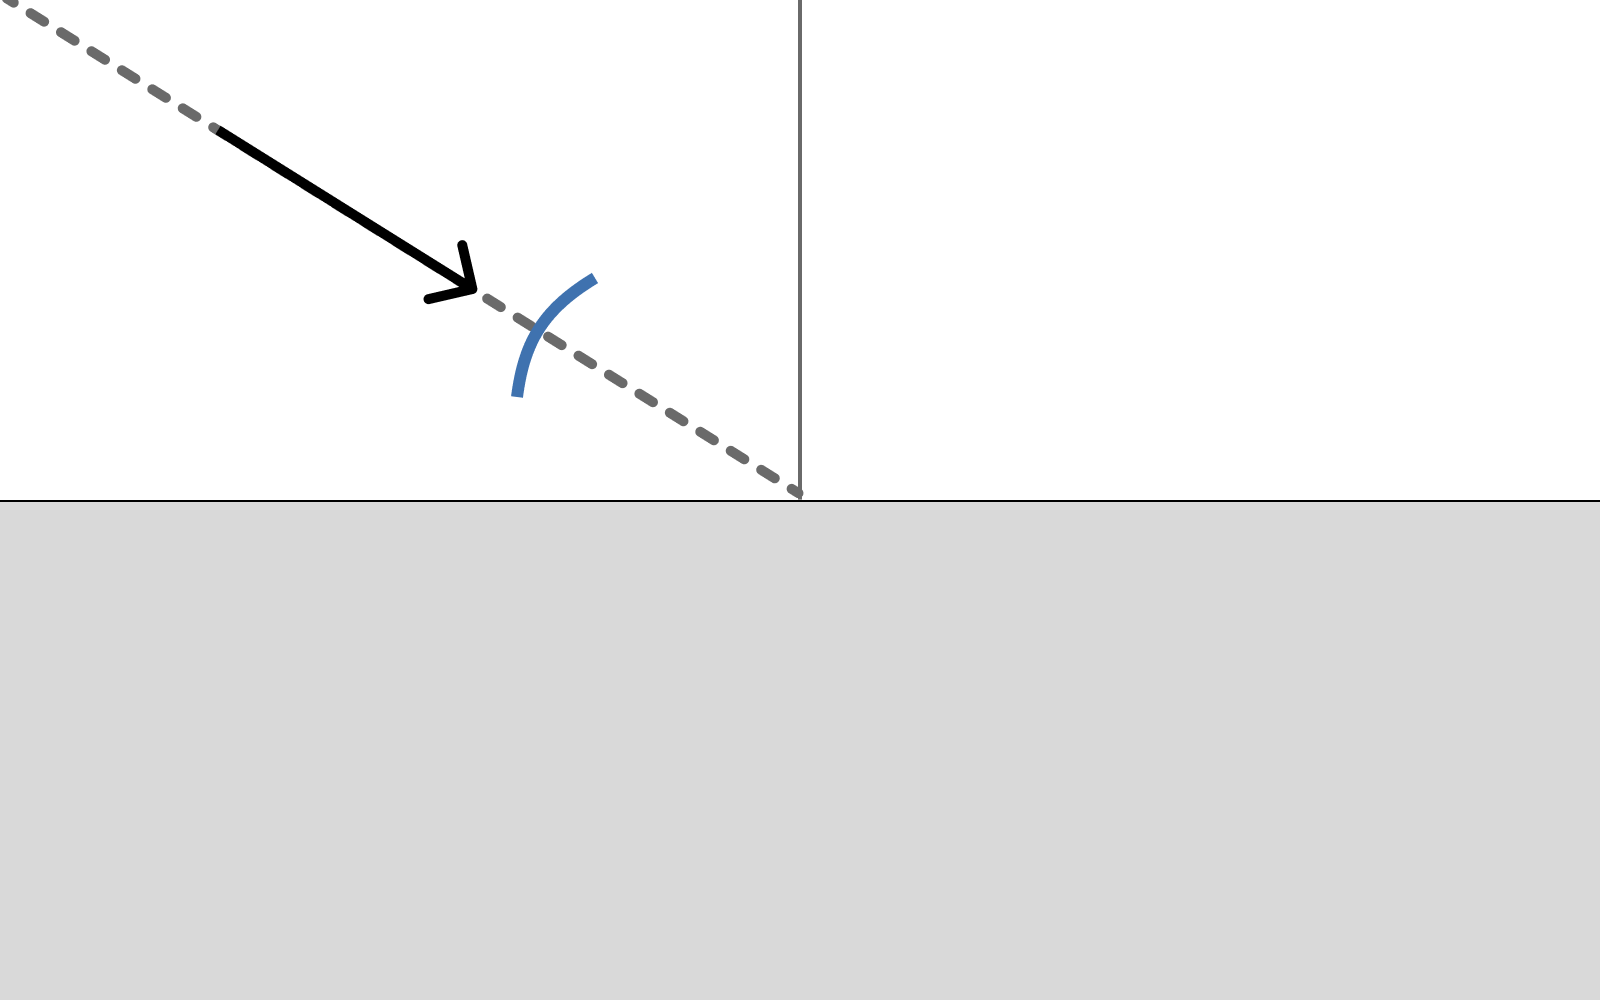
\includegraphics[width=\textwidth]{resources/reflection-retroreflective.png}
      \caption{Retroreflective reflection, as can be encountered in materials such as velvet.}
      \label{fig:reflectionRetroreflective}
  \end{subfigure}
  \begin{subfigure}[b]{0.45\textwidth}
    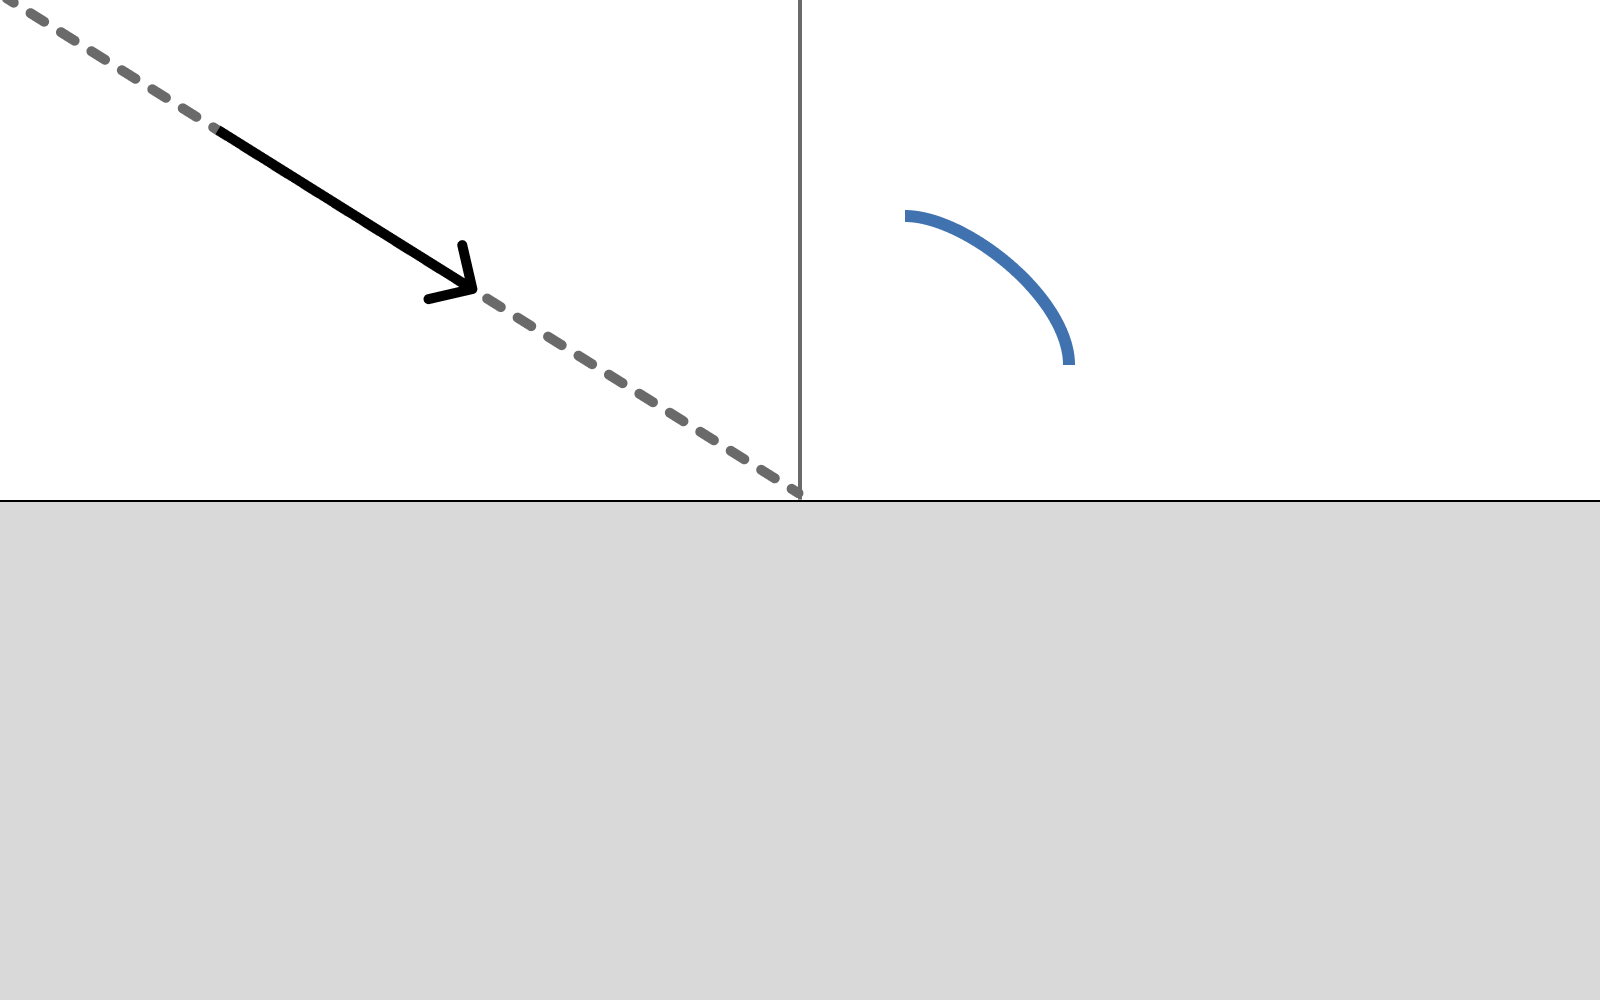
\includegraphics[width=\textwidth]{resources/reflection-glossy-specular.png}
    \caption{Glossy reflection, as can be encountered in materials such as plastic.}
    \label{fig:reflectionGlossy}
  \end{subfigure}
  \hfill
  \begin{subfigure}[b]{0.45\textwidth}
    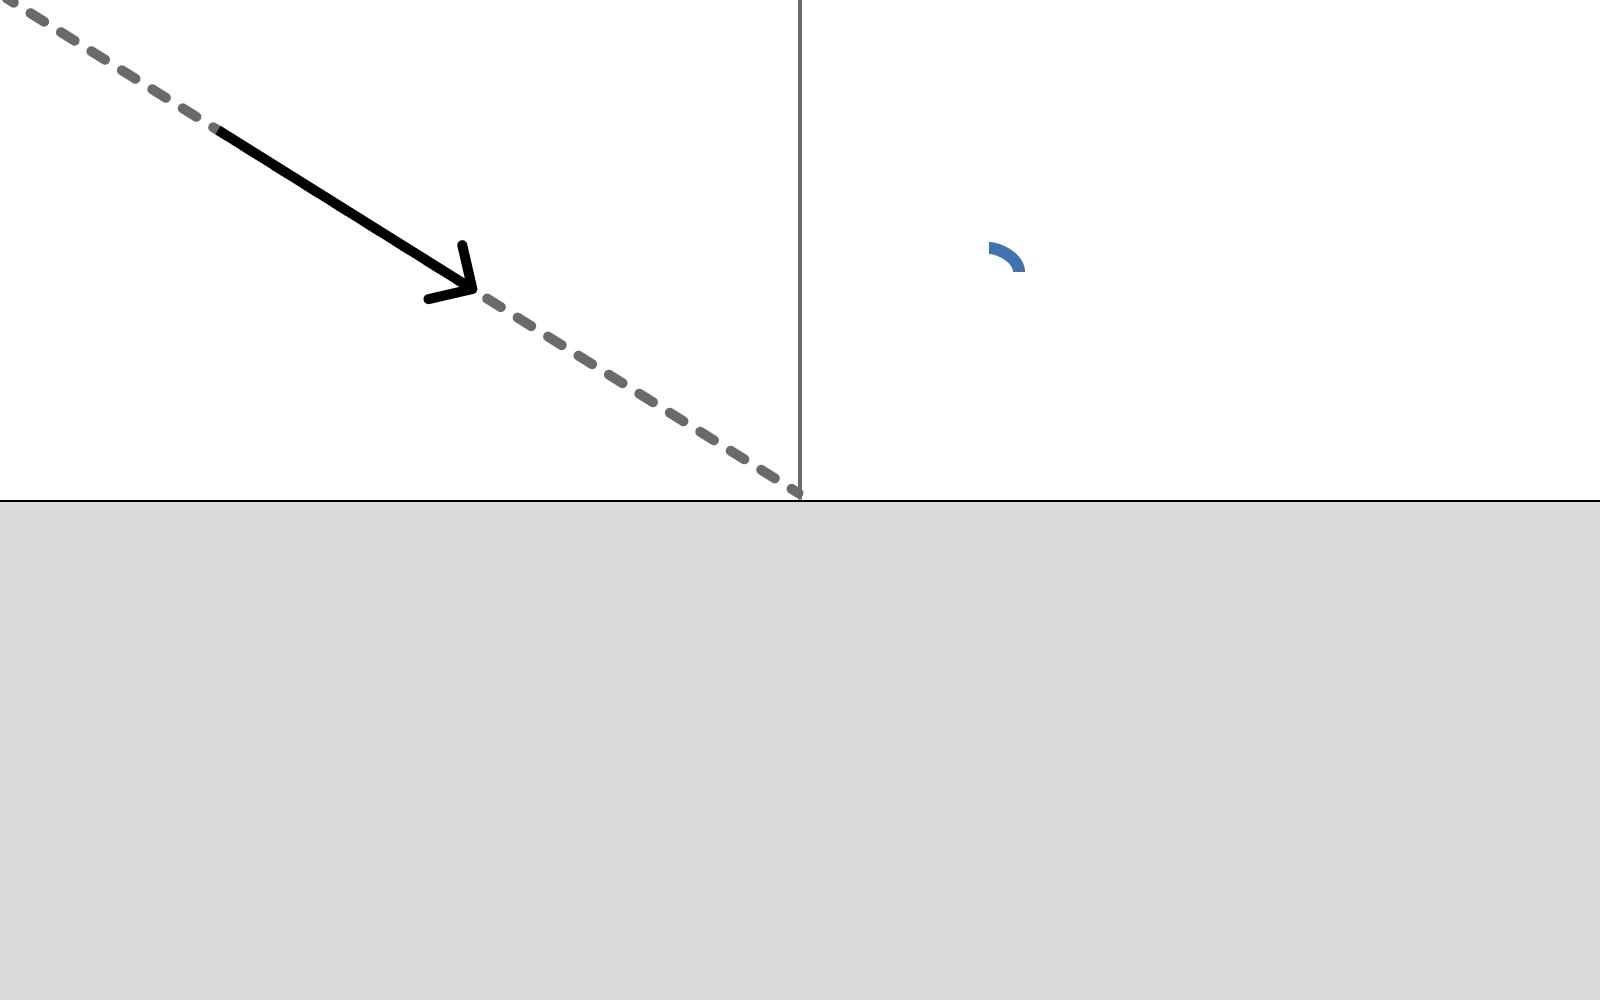
\includegraphics[width=\textwidth]{resources/reflection-specular.png}
    \caption{Specular reflection, as can be encountered in objects such as a mirror.}
    \label{fig:reflectionSpecular}
  \end{subfigure}
  \caption{Samples for different kinds of reflectance distributions. The blue line segment indicates the target of the reflection. \cite{Pharr_Physically_Based_Rendering_2023}}
  \label{fig:brdf}
\end{figure}

\subsection{Microfacet Theory}

While the macroscopic appearance of a material is visible to the human eye, the microscopic structure of the material is crucial in determining how light interacts with the material. Microfacet theory is a model which describes this microscopic structure. The distribution of the normals of the microfacet is described by a distribution function.

\subsection{Diffuse Reflection}

As early as the 18th century, Lambert described the reflection of light on a surface \cite{lambert1760photometria}. Lambertian reflection is still used as a term for diffuse reflection. The core tenant of diffuse reflection is equally scattering light in all directions, independent of the viewing angle. In 1995, Oren and Nayar suggested a novel reflection model which extended the Lambertian model to include rough surfaces \cite{oren1994generalization}, commonly known as the Oren-Nayar model.

\section{Computer Graphics Technology}

This section provides an overview of the technology used to render 3D scenes. It will introduce the hardware as well as the software used in the field with a focus on technology relevant for this thesis by introducing WebGPU and its core concepts.

\paragraph{Parallel Processing}

Sequential processing is limited in terms of performance. As the amount of data to process grows, the time to process the data grows linearly. Computer graphics exhibits a large number of problems which can be parallelized. The idea of parallelization for data processing is not new. In 1966, Flynn introduced a classification system for computer architectures based on the instruction streams and data streams they can process in parallel \cite{flynnTaxonomy,flynnTaxonomy2}. Already in 1970, Watkins described an algorithm for computer graphics leveraging a specialized processor for parallel processing \cite{surfaceAlgorithmProcessor}. Further research such as Chap, a \fGls{SIMD}{\e{Single Instruction, Multiple Data}, type of parallel processing of data points with a single instruction} graphics processor proposed in 1984 by Levinthal and Porter as part of Lucasfilm introduced a special purpose processor executing a single instruction on multiple data points \cite{chapSIMDgpu}.

\paragraph{GPU}

The first so-called consumer graphics processing units (\gls{GPU}), the GeForce 256 produced by NVIDIA \cite{evolutionOfGPU}, were developed in the 1990s and extend upon research conducted in the decades prior such as so-called superworkstations introduced by Silicon Graphics in the 1980s \cite{sigWorkstation}. These workstations were special-purpose computers which were optimized for computer graphics. The \gls{GPU} on the other hand is a specialized processor that is well-suited for workloads which require parallel processing and can be installed on a standard computer. While \gls{CPU} parallelization on consumer hardware is generally limited to a few cores, modern \glspl{GPU} have thousands of compute units which enable \gls{SIMD} processing.

Due to computational complexity, ray tracing techniques have been limited to offline rendering for a long time. Early ray tracers such as \gls{BMRT} were developed focusing on leveraging \gls{CPU} for computations. The introduction of \glspl{GPU} has lead to further research on how to optimize speed for techniques related to ray tracing. One such example of research for a well-established technique is \gls{BVH} construction on the \gls{GPU} \cite{lauterbach2009GPUbvh} instead of \gls{CPU}. Leveraging \gls{GPU} has been a focus of research and has enabled real-time ray tracing in recent years. Notable developments include reservoir-based spatio-temporal importance resampling (ReSTIR) \cite{restir} and subsequent improvements \cite{restirAdvancements,restirGeneralized}.

Nowadays GPUs are prevalent in consumer hardware such as smartphones, tablets, laptops and desktops and their use case is not limited to computer graphics. GPUs are used in a wide range of applications, such as machine learning, scientific computing and data processing. Devices, which do not have a discrete GPU, often use an integrated GPU which is part of the CPU.

Modern GPU hardware offers support for hardware-accelerated ray tracing. Examples include Nvidia RTX \cite{nvidiaRtxRayTracing}, Apple Metal on M3 \cite{appleM3GpuAdvancements} and others. These examples demonstrate an increasing trend towards hardware-accelerated ray tracing in recent years, however many devices and \glspl{API}, including WebGPU, do not yet support hardware-accelerated ray tracing.

\paragraph{Common Strategies}

Certain basic definitions have established as common practices for these \glspl{API}. The term shader is used to describe a program which runs on the \gls{GPU}. It is frequently used to describe in conjunction with different shader types which are used as part of the so-called graphics pipeline in rasterization. The pipeline in its basic form consists of two steps which are executed on the \gls{GPU} in sequence:

\begin{itemize}
    \item{Vertex Shader} — The vertex shader is responsible for transforming the vertices of the geometry into screen space. The output of the vertex shader is a set of vertices which are then rasterized.
    \item{Fragment Shader} — The fragment shader is responsible for determining the color of the fragments which are generated by the rasterizer. The fragment shader is executed for each fragment which is generated by the rasterizer.
\end{itemize}

In addition to this standard graphics pipeline, many \glspl{API} also support custom code which does not need to be used exclusively for rendering. This code can be used for general-purpose computing and is generally referred to as \gls{GPGPU}. Shaders which are used for \gls{GPGPU} are often called compute shaders.

\subsection{OpenGL}

OpenGL is an \gls{API} for rendering 3D graphics. After its introduction in 1992, it was widely adopted. Subsequently, the standard has been ported to other platforms and has been extended with new features.

To date, OpenGL is still widely used in the industry, but it has been replaced by more modern \glspl{API} in recent years.

\subsection{Vulkan, Metal, DirectX}

While OpenGL and derivatives such as OpenGL ES have been widely adopted, the introduction of a number of new \glspl{API} has changed the landscape. Some of the most notable \glspl{API} are:

\begin{itemize}
    \item{Vulkan} Developed by the Khronos Group, Vulkan is a low-level \gls{API} which is supported on a wide range of platforms.
    \item{Metal} Developed by Apple, Metal is a low-level \gls{API} which is supported on Apple platforms.
    \item{DirectX} Developed by Microsoft, DirectX is a collection of \glspl{API} which are supported on Windows platforms.
\end{itemize}

\todo{Dawn's Vulkan backend used for WebGPU on Android and ChromeOS. Plan is to use it for Linux as well (Brandon Jones).}

\subsection{WebGL}

WebGL is a graphics \gls{API} based on OpenGL ES 2.0 for the web. It was initially released in 2011 and has since been adopted by all major browsers.

WebGL is designed to offer a rendering pipeline, but does not offer \gls{GPGPU} capabilities. There have been efforts to extend with compute shaders, but efforts by the Khronos Group have been halted in favor of focusing on WebGPU instead.

In order to provide \gls{GPGPU} capabilities, workarounds have been developed. The basic idea is to render the output of a fragment shader to a texture and interpreting the output as binary data instead of color information.
There are libraries such as GPU.js which provide \gls{GPGPU} capabilities using WebGL. Tensorflow.js, a library for training and deploying Machine Learning models, use similar techniques in the WebGL backend.

Since its introduction, WebGL has been extended with new features. WebGL 2.0, which is based on OpenGL ES 3.0, was released in 2017. Of the major browsers, Safari was the last to support it out of the box in 2021. Since WebGL 2.0 no new major versions have been released but new features have been added.

\subsection{WebGPU}

WebGPU is a new web standard, being developed by \fGls{W3C}{\e{World Wide Web Consortium}, a non-profit organization dedicated to developing web standards} which is no longer based on OpenGL. One of the main capabilities is support for \gls{GPGPU} by design. While all major browser vendors have announced intent to support WebGPU, to date only Chrome has shipped WebGPU for general use on desktop as well as mobile.
The standard is still in development and new features are being added.
Common 3D engines such as \gls{Babylon.js}, \gls{Three.js}, \gls{PlayCanvas} and \gls{Unity} have announced support for WebGPU.

\subsubsection{Implementations}

Three major implementations of WebGPU exist:

\begin{itemize}
    \item{\gls{Dawn}} — Developed by Google, \gls{Dawn} is a C++ library which provides a WebGPU implementation. It is used in Chromium-based browsers \cite{dawnImplementation}.
    \item{\gls{wgpu}} — A Rust library which provides a WebGPU implementation. It is used in Firefox and \fGls{Deno}{JavaScript runtime, alternative to Node.js} \cite{wgpuImplementation}.
    \item{WebKit WebGPU} — Developed by Apple, WebKit is used in Safari \cite{webKitWebGPUImplementation}.
\end{itemize}

As the standard is under active development, there are differences between the implementations as well as the specification \cite{wgpuStandardDeviation}. Thanks to alignment and the extensive conformance test suite \cite{WebGPUConformanceTestSuite}, the implementations are largely compatible.

\subsubsection{Buffers}

Data needs to be transferred between the CPU and the GPU. Buffers are the primary method to do so. Depending on the type of data to be transferred, different types of buffers can be used.

\paragraph{Uniforms}

Uniform Buffers are optimized for data which is read-only on the GPU and is the same for all vertices or fragments. Such information could be the projection matrix.

\paragraph{Storage}

Storage Buffers are intended for read-write access on the GPU. The limits of the buffer are higher than for uniform buffers.

\paragraph{Vertex}

\paragraph{Index}

\subsubsection{Shading Language}

WebGPU introduces a new shading language called WebGPU Shading Language (\gls{WGSL}). The language is statically typed and supports a variety of data structures required for computer graphics as well as general-purpose computing.

\gls{WGSL} supports common high-level helpers such as Swizzling, which is a class of operations which facilitate managing vector elements. For example, given a vector \verb|let v = vec3f(x, y, z)|, the operation \verb|v.xy| returns a vector \verb|(x, y)|.

\subsubsection{Memory Alignment}
\label{ch:memoryAlignmentTheory}

\gls{WGSL} supports \verb|struct| for defining data structures. However, when passing data between the CPU and the GPU, memory alignment needs to be considered. Alignment is a constraint, restricting the memory address at which a data structure can be stored. Having strict memory alignment enables use of more efficient hardware instruction sets, or address hardware requirements.

Each type in \gls{WGSL} has specific alignment requirements which are independent of the size. For example, a \verb|vec3f| has a size of 12 bytes, but requires an alignment of 16 bytes. So for a struct definition such as can be seen in \autoref{code:memoryAlignment}, the struct requires 32 bytes of memory to store 20 bytes of data as illustrated in \autoref{fig:memory-alignment}. The excess 12 bytes are used for padding.

\begin{figure}[H]
  \begin{lstlisting}[style=wgsl]
  struct ThreeFields {
    a: f32,
    b: vec3f,
    c: f32
  }
  \end{lstlisting}
  \caption{\gls{WGSL} \texttt{struct} containing three fields of type \texttt{f32} and \texttt{vec3f}.}
  \label{code:memoryAlignment}
  \end{figure}

\begin{figure}[H]
  \centering
  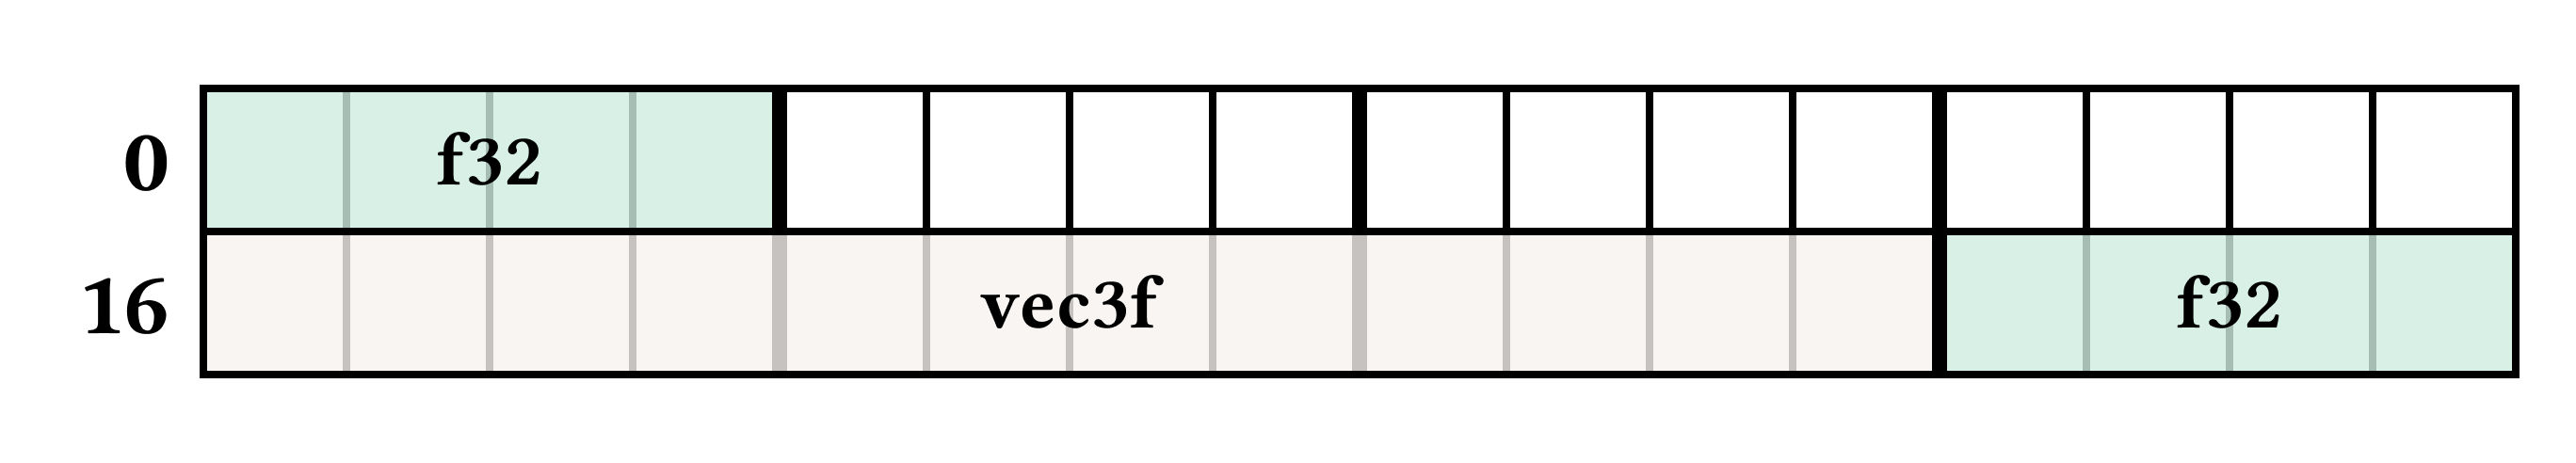
\includegraphics[width=0.8\textwidth]{resources/memory-alignment.png}
  \caption{Memory Alignment with padding for struct defined in \autoref{code:memoryAlignment}.}
  \label{fig:memory-alignment}
\end{figure}

Memory alignment is opaque while writing \gls{WGSL} code, it is relevant when providing data to the GPU. For creating buffers, the alignment requirements need to be considered. When using JavaScript to create buffers, the standard Web \glspl{API} such as \texttt{Float32Array} or \texttt{Uint32Array} can be used to provide data. In order to write data to the \texttt{struct} in \autoref{code:memoryAlignment}, the views can be created as shown in \autoref{code:memoryAlignmentJs}.

\begin{figure}[H]
  \begin{lstlisting}[style=JavaScript]
const ValueBuffer = new ArrayBuffer(32);
const a = new Float32Array(ValueBuffer, 0, 1);
const b = new Float32Array(ValueBuffer, 16, 3);
const c = new Float32Array(ValueBuffer, 28, 1);
  \end{lstlisting}
  \caption{JS code providing views to access the \texttt{struct}.}
  \label{code:memoryAlignmentJs}
\end{figure}


\section{Exchange Formats}

In order to exchange 3D scenes between a multitude of applications, various standardized formats have been developed. These formats are optimized for different use cases depending on the requirements of the application. For the purpose of this thesis, the focus is on formats which are well-suited for real-time rendering on the web. In comparison to other use cases, certain aspects are more important on the web. These aspects include:

\begin{itemize}
    \item{Efficiency} – It should be optimized for transmission and loading. While data compression algorithms such as gzip can alleviate some of the issues during transmission, pure text-based formats are generally less efficient than binary formats.
    \item{Feature Set} – The format should support a wide range of features such as geometry, materials and scene graph.
    \item{Interoperability} – The format should be widely supported by 3D engines and applications.
\end{itemize}

The following section categorizes the formats based on their use case and highlights some of the most widely known formats.

\subsection{General Purpose Formats}

One of the most widely used formats is Wavefront \gls{OBJ} which was established in the 1980s. The format is text-based and has basic support for materials and textures via a companion file \fGls{MTL}{\e{Material Template Library}, a companion file format to \gls{OBJ} for material definitions}. However, it lacks support for more advanced features such as animations. Additionally, due to its encoding, it is not well-suited for delivery over the web compared to more modern alternatives.

Formats such as the proprietary FBX by Autodesk established in 2006 can address the shortcomings in terms of advanced features. The format is supported by a wide range of applications. One of the main disadvantages is the proprietary nature of the format  which can make it difficult to integrate in a applications which do not have access to the SDK.

\subsection{Specialized Formats}
\label{ch:specializedFormats}

For specific use cases, specialized formats have been developed. One such example is \gls{STEP} which is standardised in ISO 10303. The format is widely used in product manufacturing and offers support for a wide range of modelling features. The \fGls{ASCII}{\e{American Standard Code for Information Interchange}, character encoding standard for electronic communication} encoding of the format is human-readable but is not well suited for real-time rendering requirements of the web due to transmission size and parsing complexity \cite{marjudi2010StepIgesreview}. Parsing complexity is exhibited by the large number of different entities which can be defined in the format.

Another such format is STL which is widely used in 3D printing and supports binary as well as \gls{ASCII} encoding. It lacks support for advanced features such as material representation, animations and scene graph.

\subsection{Interoperability Formats}

The aforementioned formats have shortcomings in terms of interoperability and feature set for complex 3D scenes. Special formats have been developed to address issues encountered in complex 3D scenes such as encountered in the film industry.

Other formats such as COLLADA have been developed to improve transporting 3D scenes between different applications. It is XML-based and has been established in 2004 and has since been managed by the Khronos Group. The latest release of the format was in 2008.

One notable format is USD, which has been open-sourced by Pixar in 2016. Similar to COLLADA, the format is designed with interoperability in mind. The main focus of USD is support for complex scenes and complex collaboration workflows. The format is widely supported by 3D engines and applications.

\subsection{Runtime Formats}

For usage in end-user applications, such as for the use cases in this thesis, the \gls{glTF} format is well-suited. It has been established in 2015 and is designed to be efficient for transmission and loading of 3D scenes. The standard is developed by the Khronos Group and is widely supported by 3D engines and applications. The format supports 3D geometry, materials, animations, scene graph and other features.

Technically, the format offers two different encoding formats which differ in file ending:

\begin{itemize}
    \item{\texttt{.glb}} – Binary format which is optimized for transmission and loading.
    \item{\texttt{.gltf}} – Text-based format which is human-readable.
\end{itemize}

\gls{glTF} is designed to be extensible and a variety of extensions have been developed to support features such as mesh compression using Draco.

The hierarchy structure of a \gls{glTF} file is shown in \autoref{fig:gltf-hierarchy}.

\begin{figure}[H]
  \centering
  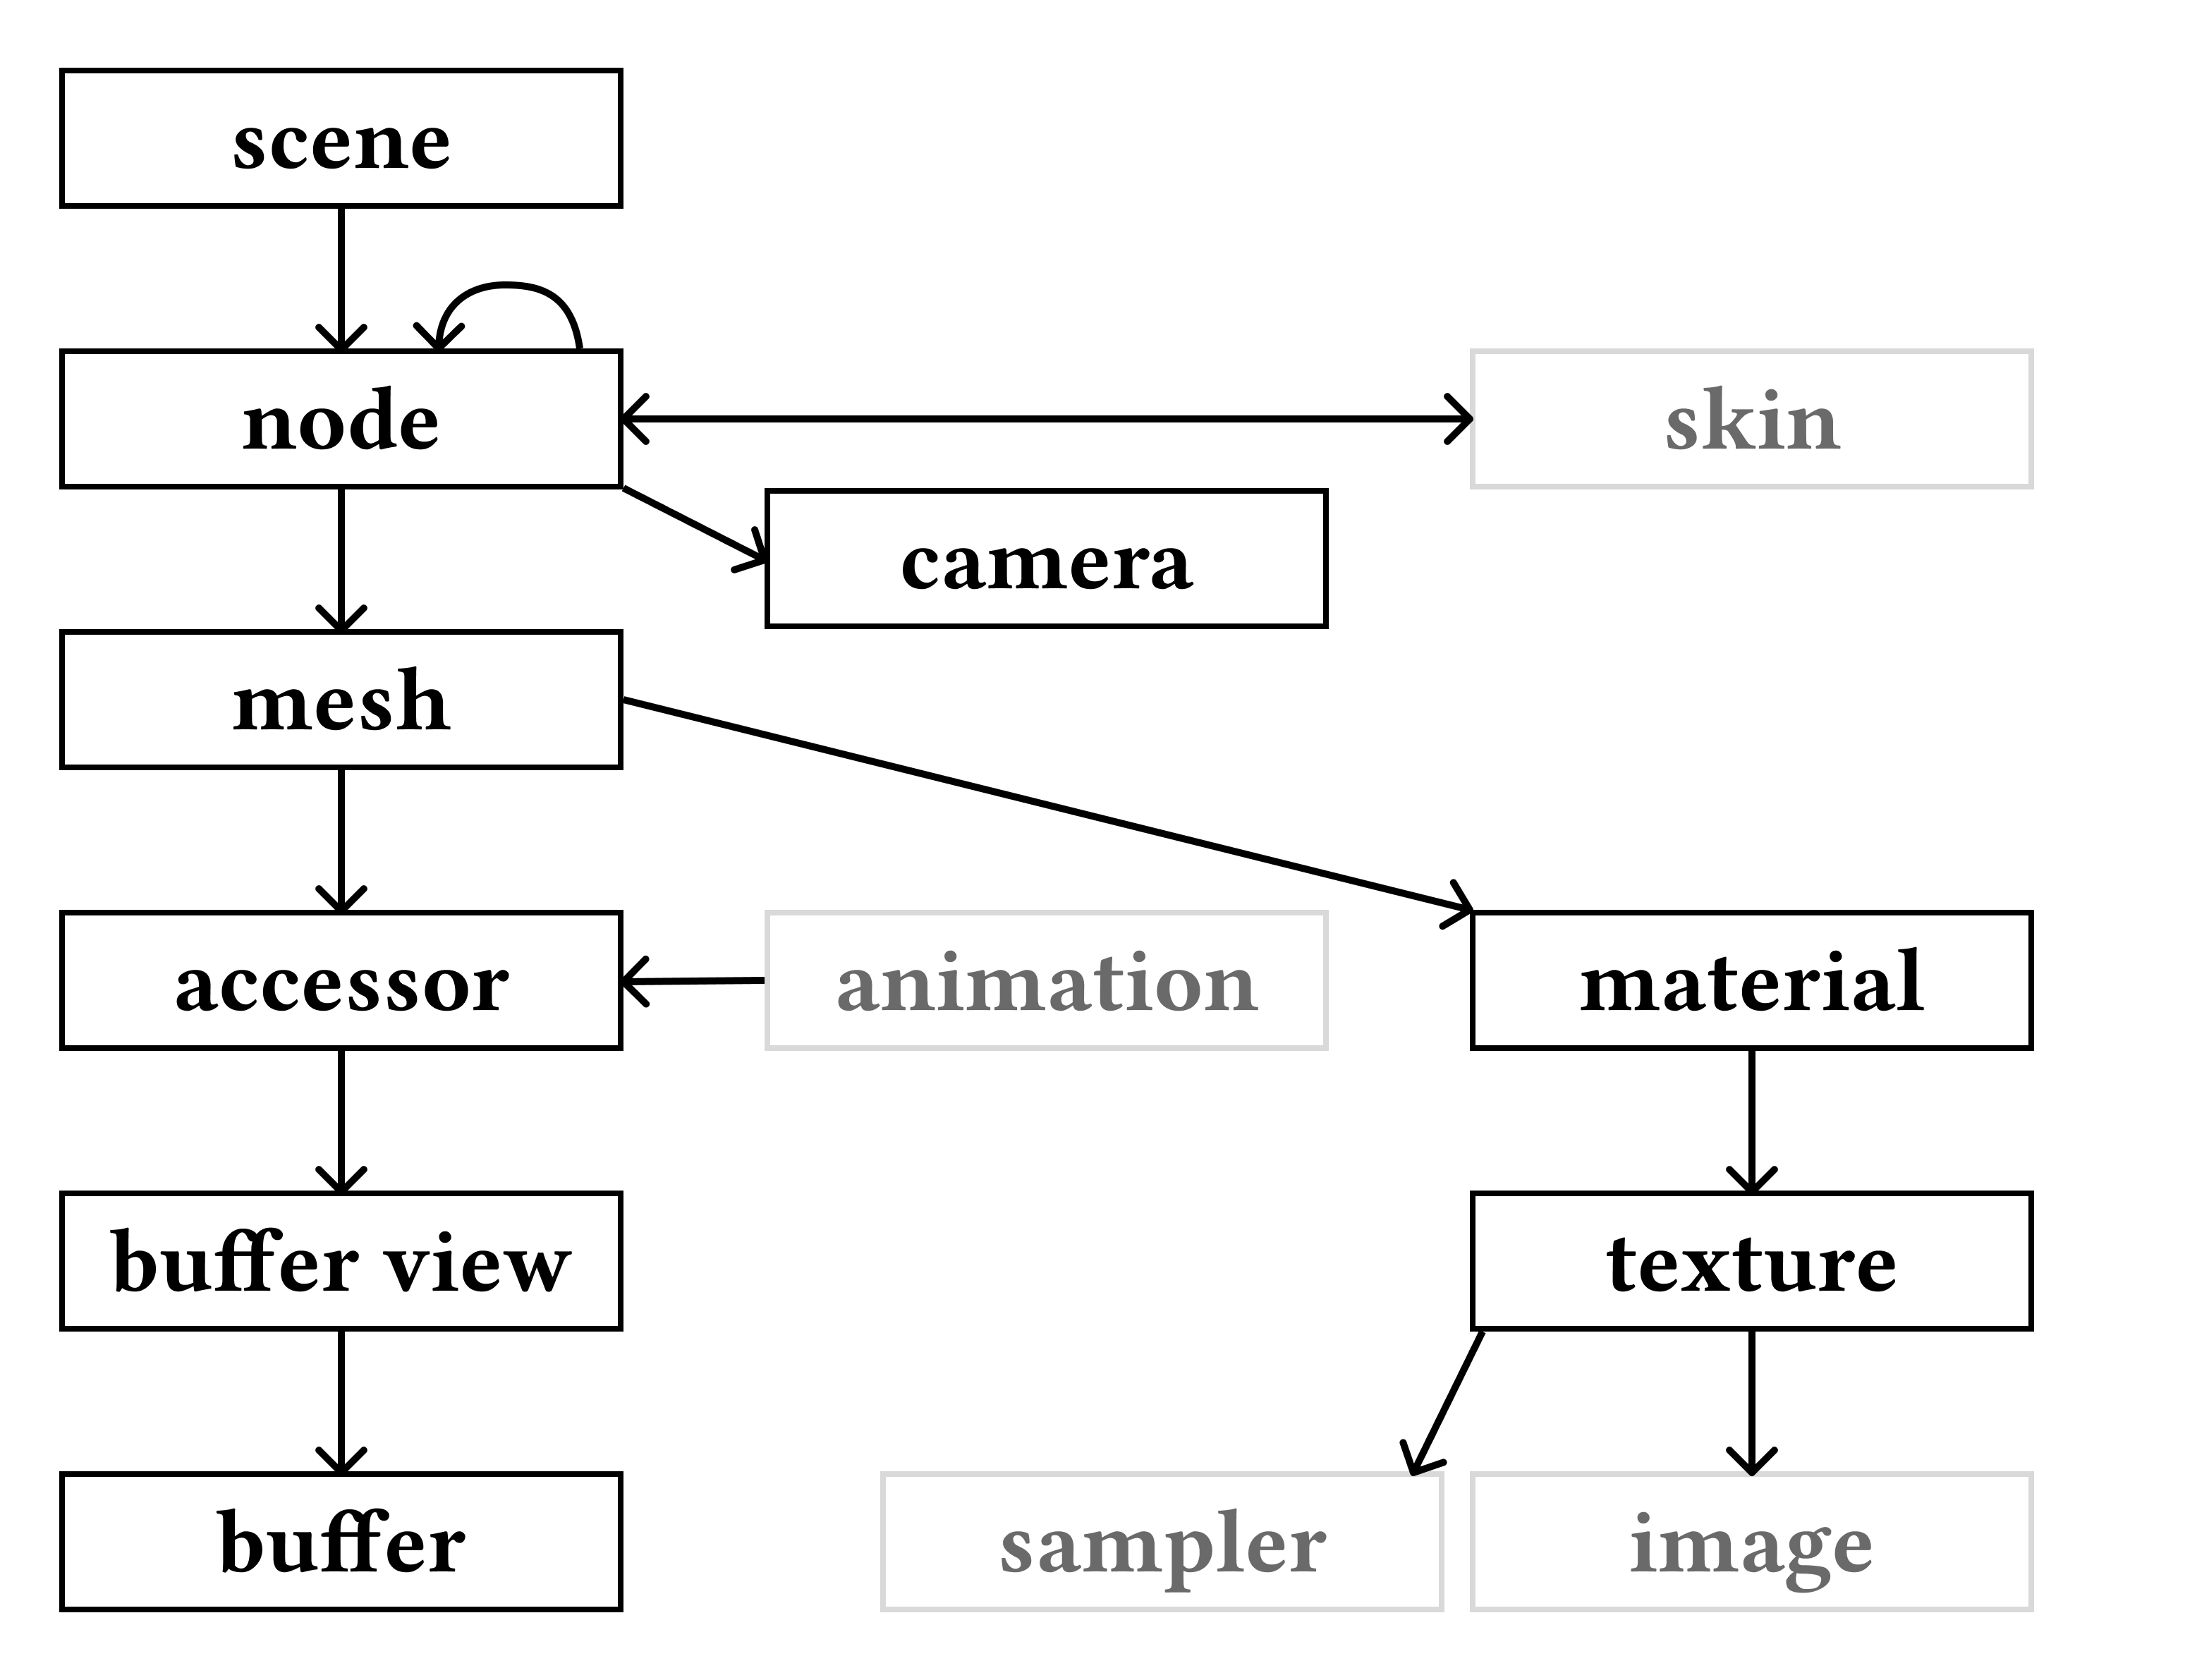
\includegraphics[width=0.6\textwidth]{resources/gltf-hierarchy.png}
  \caption{glTF hierarchy starting with the \texttt{scene} object. Arrows indicate parent-child relationships. Gray objects are not mentioned in this thesis.}
  \label{fig:gltf-hierarchy}
\end{figure}

\section{Material Description}

While the principles of \gls{PBR} are well-established, the material description in 3D formats is not uniform. A variety of different approaches have been developed. In addition to many exchange formats such as \gls{glTF} having their own material definition, different shading models exist independent of these formats. Similar to exchange formats, a variety of different use cases are addressed by material description models. While some shading models are optimized for real-time rendering, others are optimized for film production.

Many exchange formats, such as \gls{glTF}, support material description as part of the standard. The material description in \gls{glTF} supports a \gls{PBR} approach which is based on the metallic-roughness material model \todo{source?}. However, the \gls{PBR} material description in \gls{glTF} is limited in terms of feature set, by lacking features such as subsurface scattering, and is not intended to become an open standard across a variety of applications.

In addition, many real-time rendering engines such as Unity and Unreal, modeling software such as 3ds Max and Maya have their own shading models. Supporting many different shading models in a web-based real-time rendering application can be challenging, making the need for a common material description standard more apparent. This is where new material description standards come into play. These are open standards intended to be used across different applications.

\paragraph{Shader Design}

Material description models differ in how they need to be implemented. Flexible node-based systems permit the creation of custom shaders. This gives a lot of possibility to the user. The underlying implementation needs to convert the node graph into shader code which can be executed on the \gls{GPU}. In addition, managing a large number of custom shaders can be challenging as many shaders have similar features.

An alternative approach is to use an \gls{uber shader}. The term does not have a strict definition, but generally it is used to describe a shader program which can be adjusted using parameters to achieve different looks. The shader program is fixed and does not allow for customization of the shader graph. This approach often leads to a more complex shader with many parameters which can be difficult to manage.

Technically, a node-based system also supports an \gls{uber shader} approach, but a \gls{uber shader} does not support a node-based system.

\subsection{MaterialX}

\gls{MaterialX} is an open standard which was originally developed by Lucasfilm in 2012. The standard has since been adopted by the Academy Software Foundation as an open standard.

While not strictly limited to \gls{PBR}, the standard provides a wide range of features to describe physically based materials \cite{Harrysson2019}.

\gls{MaterialX} supports extensive shader generation capabilities. This permits to re-use shaders across different applications and frameworks and aids in understanding the used approximations.

\subsection{OpenPBR}

\gls{OpenPBR}\cite{openPBRSpec} is a surface shading model hosted by the Academy Software Foundation as an open standard. It differs from \gls{MaterialX} in that it is providing an \gls{uber shader} approach instead of a node-based approach. Version 1.0 of the standard was released in June of 2024 \cite{openPBR1Dot0Release}.

It serves as a combination of Autodesk Standard Surface and Adobe Standard Material and is being worked on by both companies. The potential of this standard is to provide a common shading model which can be used across different applications. One notable adopter of the standard is Nvidia Omniverse, which has shipped support of the standard \cite{omniverseOpenPBR}. Blender has reworked their Principled BSDF shader to be based on \gls{OpenPBR} \cite{blenderOpenPBRInspiration}. These promising signs indicate that the standard has the potential to be widely adopted.

The \gls{uber shader} approach is defined by having a fix set of inputs which can be adjusted, but it does not allow for custom node graphs as \gls{MaterialX} does. The standard is designed for photorealistic material description and uses multiple layers to describe the material as visualized in \autoref{fig:openPBR}.

\begin{figure}[H]
  \centering
  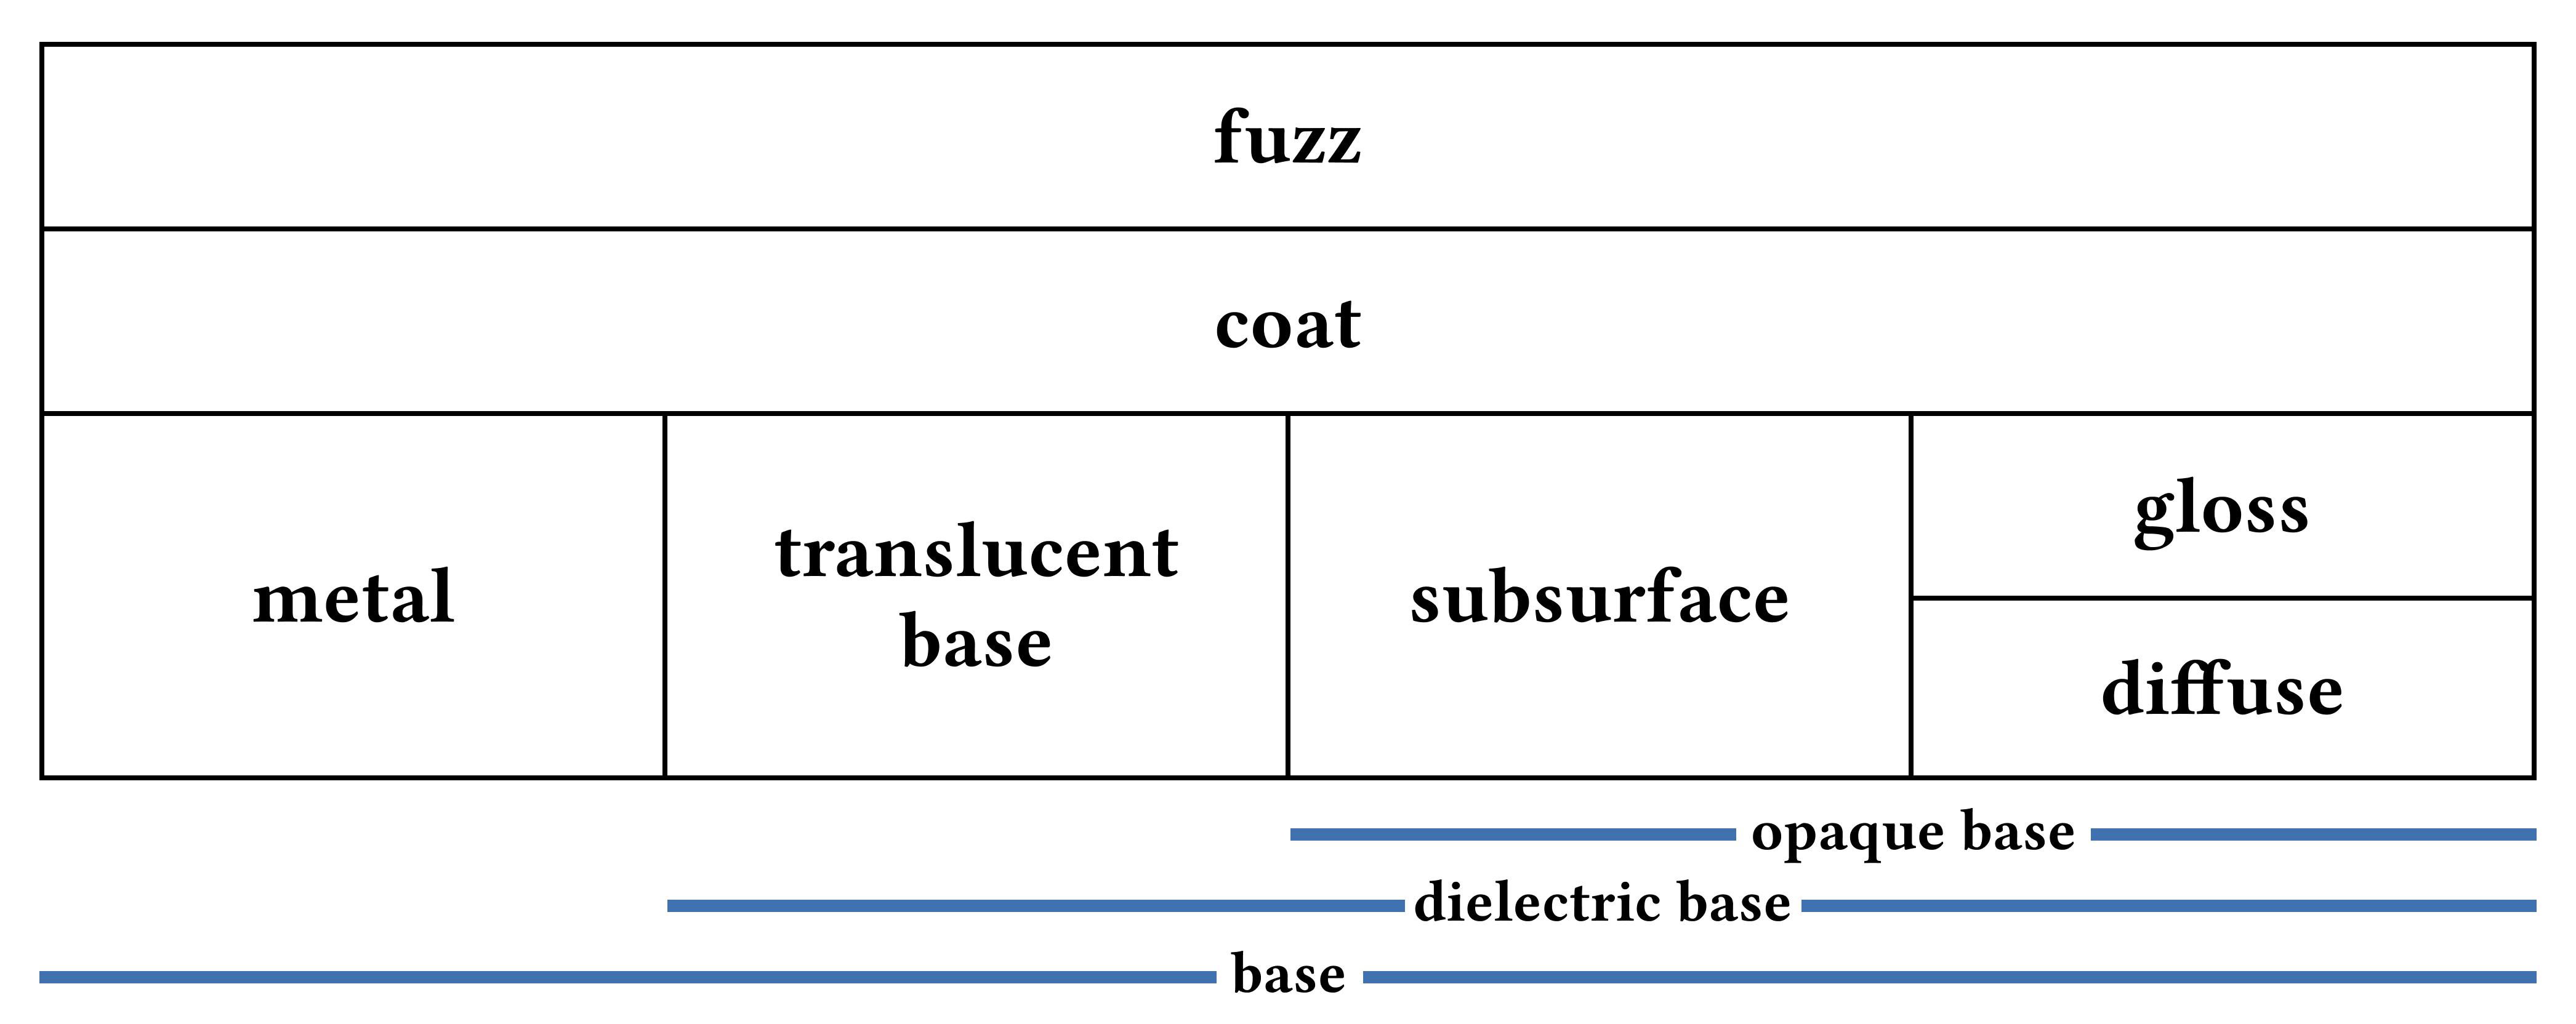
\includegraphics[width=0.5\textwidth]{resources/openpbr.png}
  \caption{The different layers of the \gls{OpenPBR} shading model.}
  \label{fig:openPBR}
\end{figure}

The \gls{OpenPBR} specification includes a reference implementation in \gls{MaterialX}. This allows to use the shader generation of \gls{MaterialX} in order to get a reference shader implementation for \gls{OpenPBR}.
